% !TEX root = ../main.tex

\chapter{基准分割模型3D-UNet和分割效果分析}

\section{医疗图像语义分割基础}

图像的语义分割是一种像素级的分类技术,输入一张(RGB彩色或灰度)图片,分类器输出图片上每一个像素所属的类别标签。基于深度
学习的图像语义分割方法,其主要算法是卷积神经网络(Convolutional Neural Network, CNN)。卷积神经网络通常包含以下四层:
\begin{itemize}
    \item 卷积层 Convolution layer
    \item 归一化层 Normalization layer
    \item 激活函数层 Activation function
    \item 池化层 Pooling layer
\end{itemize}
CNN的基本网络结构如图\ref{fig:CNN_basic_structure}所示:
\begin{figure}[!htp]
    \centering
    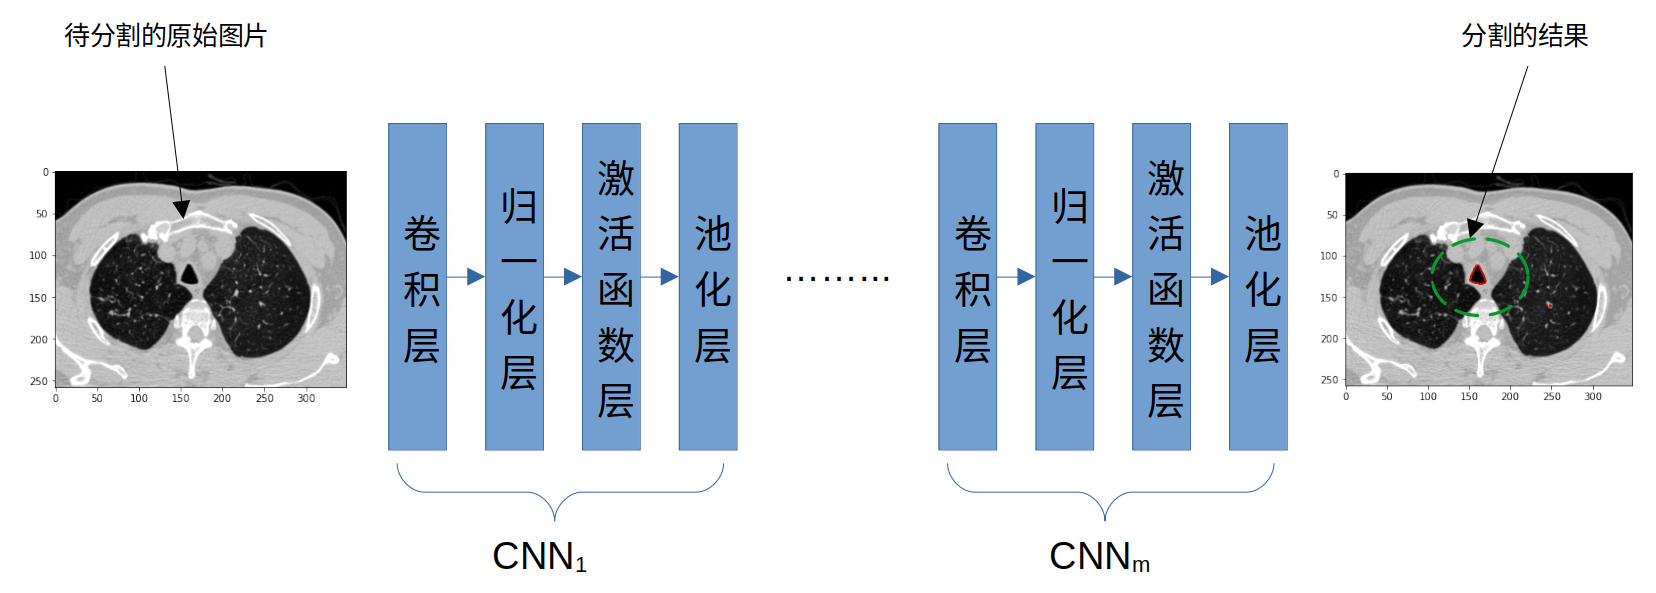
\includegraphics[width=\textwidth]{CNN_Structure}
    \bicaption[卷积神经网络基本构成]
        {卷积神经网络基本构成}
        {The basic structure of CNN}
    \label{fig:CNN_basic_structure}
\end{figure}

\noindent{}待分割的原始图片经过一层或连续多层的卷积网络后,图片的低层位置信息与高层语义信息等被提取出来,最后得到分割的结果。每次迭代
将预测的结果与真实的分割结果进行对比,选取一个合适的损失函数,计算损失值。然后通过梯度下降的反向传播,对卷积网络的参数---也就是
网络中每个神经元的权重Weight与偏置Bias---进行更新。循环进入下一次迭代,直到损失值不再降低趋于平缓,网络收敛,整个训练过程完成。

\subsection{卷积层}
卷积层的主要作用是提取特征,获得图像的局部信息。其工作原理是:在输入图像上滑动$H \times W = 3 \times 3$的窗口,每滑动
1个单位长度(此处滑动的长度称为步长Stride)就提取这个$3 \times 3$窗口内的像素信息,与同样尺寸的一个权重矩阵
(亦即卷积核尺寸convolution kernel size)做点积相乘并求和,得到当前位置的特征。

令$H3 \times W3$卷积核权重矩阵$W_{conv.kernel}$
\begin{equation}
    W_{conv.kernel} = \begin{bmatrix}
        w_1 & w_2 & w_3 \\
        w_4 & w_5 & w_6 \\
        w_7 & w_8 & w_9
    \end{bmatrix}
\end{equation}

CT扫描图像在$H3 \times W3$窗口内的Hounsfield unit\cite{HU2016CT}灰度\footnote{Hounsfield unit亨氏单位
是放射科医生在解释CT图像时使用的相对定量的无线电密度测量单位。CT重建时使用身体组织对辐射的吸收/衰减系数来生成灰度图像。
身体组织的物理密度与X射线束的吸收/衰减成正比。Hounsfield单位,也称为CT单位,是根据X射线束的线性衰减系数进行线性
变换计算而来的。}像素矩阵$X_{hu.gray}$
\begin{equation}
    X_{hu.gray} = \begin{bmatrix}
        x_1 & x_2 & x_3 \\
        x_4 & x_5 & x_6 \\
        x_7 & x_8 & x_9
    \end{bmatrix}
\end{equation}
则当前位置的特征$feat(X)$为
\begin{equation}\label{eq:conv}
\begin{split}
    {feat}(X) &= \sum{\left(W \cdot X\right)} + b \\
            &= \sum{\left(\begin{bmatrix}
                        w_1 & w_2 & w_3 \\
                        w_4 & w_5 & w_6 \\
                        w_7 & w_8 & w_9
                    \end{bmatrix} \cdot 
                    \begin{bmatrix}
                        x_1 & x_2 & x_3 \\
                        x_4 & x_5 & x_6 \\
                        x_7 & x_8 & x_9
                    \end{bmatrix}\right)} + b
\end{split}
\end{equation}
其中$b$为偏置参数Bias

式\ref{eq:conv}是在二维图像平面上的卷积操作,若在CT三维体数据上进行卷积运算,则卷积核尺寸扩展为$D3 \times H3 \times W3$
,相应地Hounsfield unit灰度像素矩阵也同步扩展到三维。三维卷积的操作如图\ref{fig:3D_Conv}所阐述:
\begin{figure}[!htp]
    \centering
    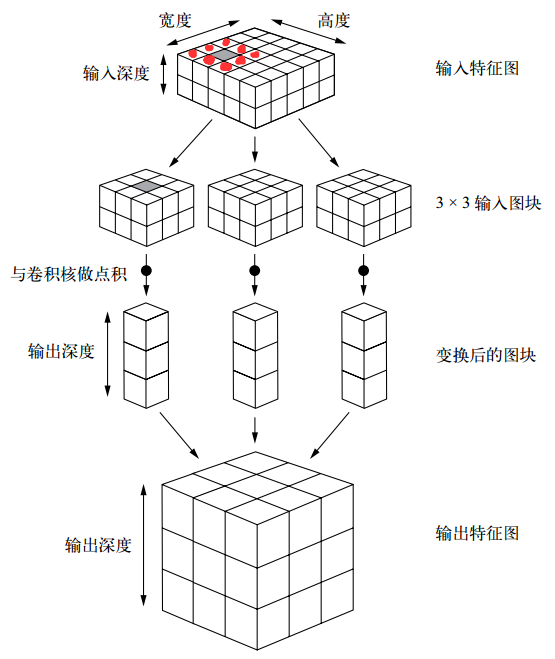
\includegraphics[width=0.5\textwidth]{Convolution_pricinple}
    \bicaption[三维卷积操作的原理]
        {三维卷积操作的原理}
        {The principle of 3D convolution}
    \label{fig:3D_Conv}
\end{figure}

\subsection{归一化层}
训练深度神经网络的计算强度非常大,训练时间漫长。减少训练时间的一种方法就是使网络中的神经元的活动归一化\cite{Ba2016LayerN}。
归一化是沿着某个指定的维度计算特征的均值与方差,对于推动深度网络收敛有着非常重要的作用。我们常用的归一化有:
\begin{enumerate}
    \item {批次归一化 Batch Normalization\cite{Ioffe2015BatchNA}}
    
    批次归一化是沿着Batch维度计算特征的均值和方差来进行归一化,批次的大小Batch size决定着预测的误差。通常取更大一些的Batch size
    有利于降低误差。过小的Batch size会导致性能下降。
    \item {层次归一化 Layer Normalization\cite{Ba2016LayerN}}
    
    层次归一化是沿着Channel维度计算特征的均值和方差来进行归一化。因为批次归一化依赖于Batch size, 尤其是不能低于mini batch size,
    而层次归一化是为了克服此问题的。
    \item {实例归一化 Instance Normalization\cite{Ulyanov2016InstanceNT}}
    
    实例归一化跟批次归一化执行相同的计算,但却是对单个样本而言。实例归一化可用于防止特定实例的均值和协方差偏移,简化学习过程。
    \item {群组归一化 Group Normalization\cite{Wu2018GroupN}}
    
    群组归一化是把Channel切分为组,在每个组内计算特征的均值和方差。群组归一化被Wu Yuxin等人\cite{Wu2018GroupN}提出来
    用于替换批次归一化,不同于层次归一化与实例归一化的方式,解决批次归一化对Batch size依赖的问题。
\end{enumerate}
我们可以用图\ref{fig:4norm}来讲解这4种归一化方式的差别。
\begin{figure}[!htp]
    \centering
    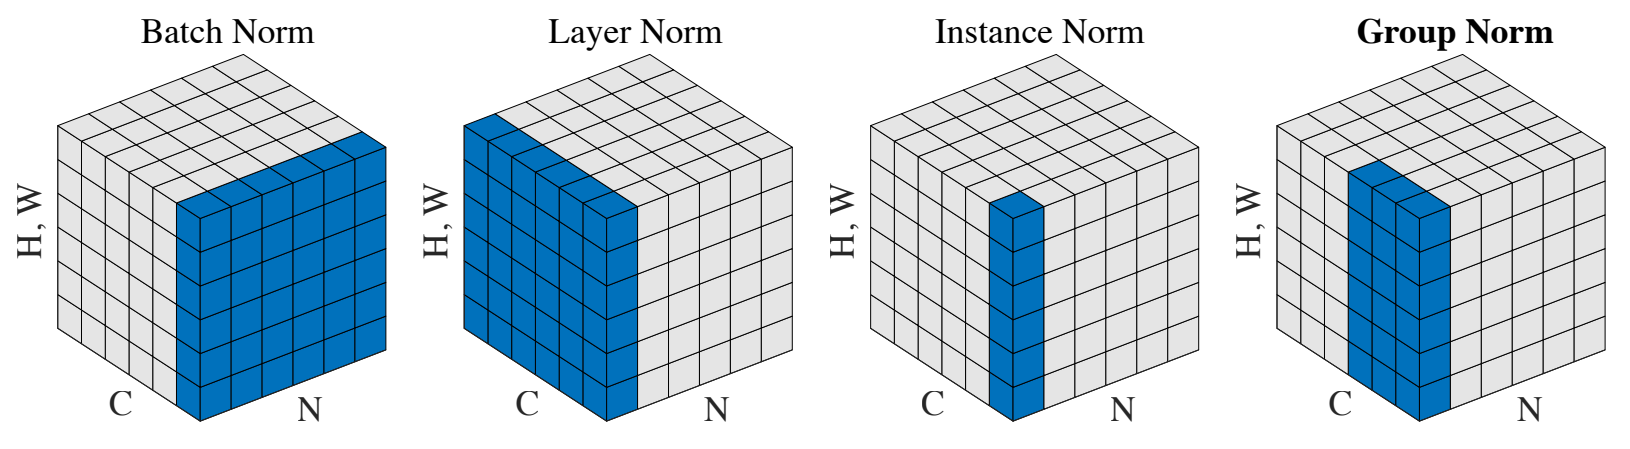
\includegraphics[width=\textwidth]{Four_Normalization_Methods}
    \bicaption[四种归一化方法的差别]
        {四种归一化方法\cite{Wu2018GroupN}}
        {Four Normalization Methods}
    \label{fig:4norm}
\end{figure}
深度网络的数据维度一般是$[Batch, Channel, Height, Width]$,简写为$[N, C, H, W]$($N$即为$Batch$)。
因为这是四个维度,我们无法画出一个四维空间的图形,所以压缩特征的$H, W$至一个维度。

\noindent{}批次归一化Batch Normalization沿Batch维度计算特征的均值和方差,归一化为$[N, H, W]$的维度,如图\ref{fig:4norm}
的Batch Norm子图的蓝色方格所示。

\noindent{}层次归一化Layer Normalization避开Batch维度,而是沿Channel维度计算特征的均值和方差,归一化为$[C, H, W]$的维度,
如图\ref{fig:4norm}的Layer Norm子图的蓝色方格所示。

\noindent{}实例归一化Instance Normalization选择单个样本计算特征的均值和方差,单个样本(也即一张图片)的维度只有$Height$
与$Weight$,所以归一化$[H, W]$的维度,如图\ref{fig:4norm}的Instance Norm子图的蓝色方格所示。

\noindent{}群组归一化Group Normalization则是介于层次归一化和实例归一化之间,其将$Channel$维度切分为很多组$Group$,
在每一个组内计算特征的均值和方差,归一化为$[C//G, H, W]$的维度,如图\ref{fig:4norm}的Group Norm子图的蓝色方格所示。

此外还有权重标准化(Weight Standardization\cite{Qiao2019WeightS})、 
批次-通道归一化(Batch-Channel Normalization\cite{Qiao2019RethinkingNA})、
深度归一化(DeepNorm\cite{Zare2017DeepNormADL})三种归一化方法,在此不做深入介绍。

\subsection{池化层}
池化的作用是缩小图像在高度和宽度方向上的空间运算,是一种降维的操作,可以用来改变当前层的输出维度,增大感受野。 池化有两种方式:
最大化池化Max Pooling和平均池化Average Pooling。最大化池化是从目标区域(图\ref{fig:pooling}的红色区域)中取出最大值,
平均池化则是计算目标区域(图\ref{fig:pooling}的深蓝色区域)的平均值。
\begin{figure}[!htp]
    \centering
    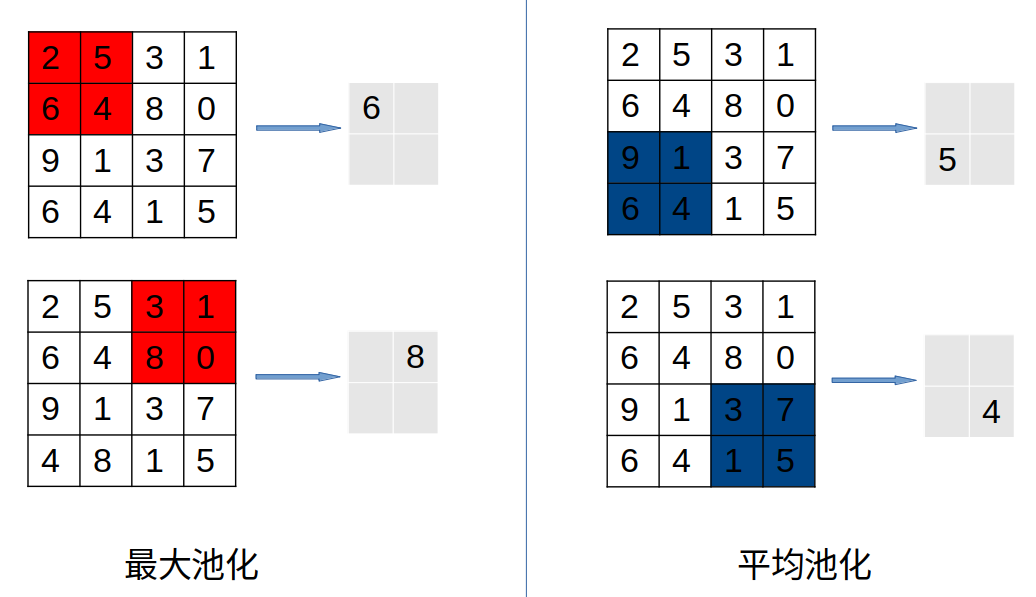
\includegraphics[width=0.7\textwidth]{Pooling}
    \bicaption[池化操作]
        {池化的基本操作}
        {The basic operations of pooling}
    \label{fig:pooling}
\end{figure}

池化层具有如下2个特征:
\begin{enumerate}
    \item {\heiti 没有要学习的参数}
    
    池化层与卷积层不一样,它没有要学习的参数。池化只是计算目标区域内的最大值或者平均值,所以不存在参数需要学习而改变。
    \item {\heiti 卷积的通道数保持不变}
    
    经过池化层,输入数据跟输出数据的通道数保持不变,是按照通道独立计算的。
    \begin{figure}[h]
        \centering
        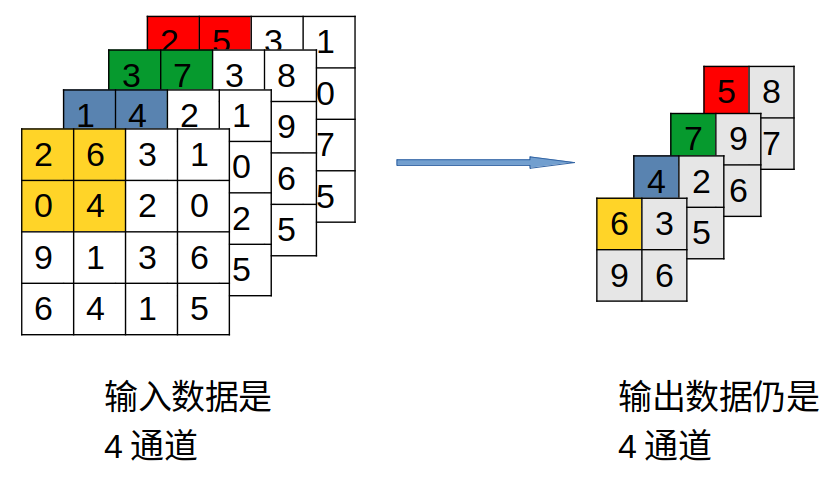
\includegraphics[scale=0.3]{Pooling_channels}
    \end{figure}
\end{enumerate}


\section{3D-UNet基准模型}
本文我们采用3D-UNet\cite{cciccek20163d}网络结构模型来分割支气管气道树,3D-UNet网络是将经典的UNet\cite{ronneberger2015u}
网络从平面图像分割扩展到三维体数据的。跟UNet网络的U型结构相似,我们将卷积层换成3D卷积,归一化层换成3D归一化,相应地池化层也更换为3D池化。
CT图像是一种体数据形式,它由一层一层的切片堆叠而成,每一层切片是一张二维的灰度图像。相比于平面图像中的像素,在CT图像中我们
定义体素Voxel为$D \times H \times W = 1 \times 1 \times 1$的立方体所含的像素,$D = 1$表明是一层切片。3D-UNet
网络的输入是$D \times H \times W$的体数据,我们称之为Cuboid,输出是每个体素的二分类分割概率图。我们在下采样路径上设计
4个卷积层块,每个卷积层块包含2层卷积。而在上采样路径上同样设计4个反卷积层块,每个反卷积层块包含2层反卷积。

\subsection{网络结构设计}

下采样路径上,每个卷积层块的结构如图\ref{fig:convblock}所示,将输入的体数据图像的通道数扩增一倍,从输入的$n$个特征通道
扩增到$2n$个特征通道。经过3D最大池化后,分辨率降低一半。
\begin{figure}[h]
    \centering
    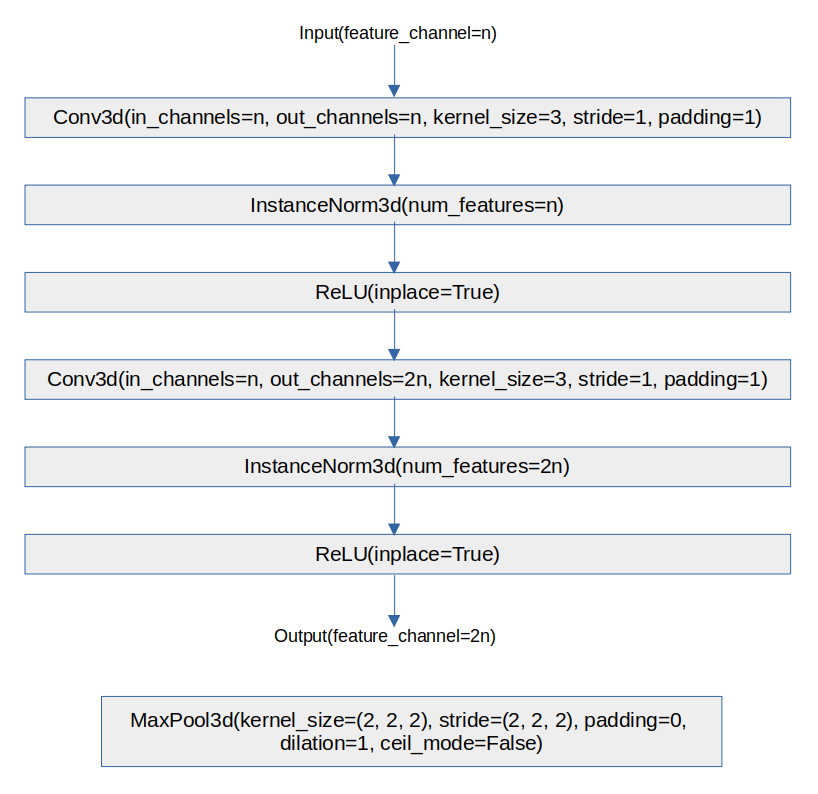
\includegraphics[width=0.8\textwidth]{Down_Conv_block}
    \bicaption[3D-UNet下采样路径上卷积层块和池化层的结构]
        {3D-UNet下采样路径上卷积层块和池化层的结构}
        {The convolution block and pooling layer in the down-sampling path of 3D-UNet}
    \label{fig:convblock}
\end{figure}

在上采样路径上,每个反卷积层块的结构如图\ref{fig:deconvblock}所示,将输入的体数据图像的通道数缩减一半。从输入的$n$个特征
通道缩减到$\frac{n}{2}$个特征通道。经过上采样池化后,分辨率升高一倍。将下采样路径降低的分辨率恢复起来,这样就实现端到端,
体素到体素的分割。
\begin{figure}[h]
    \centering
    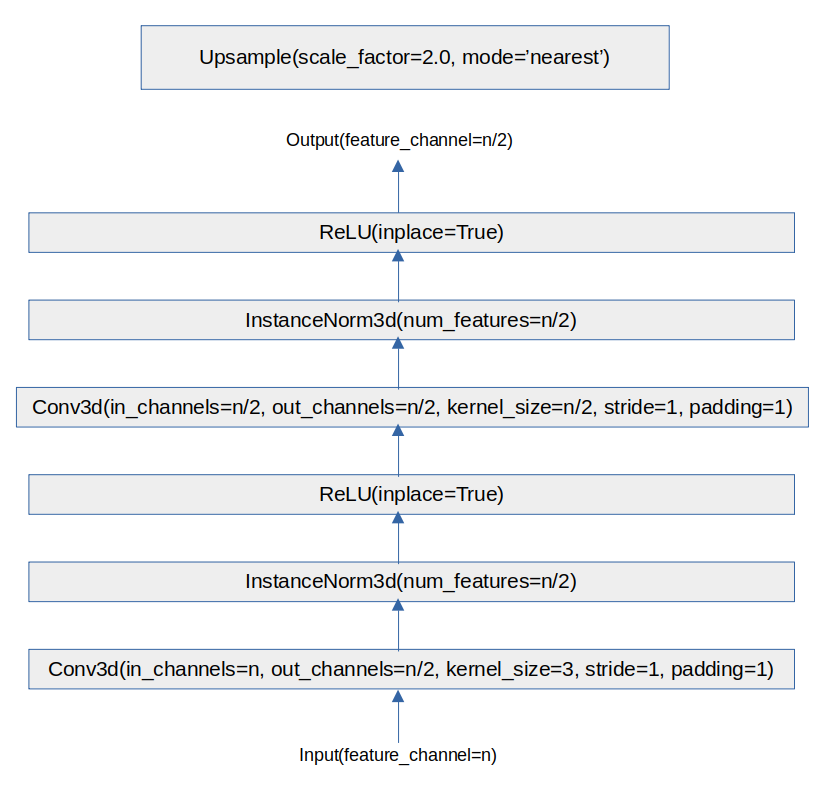
\includegraphics[width=0.8\textwidth]{Up_Conv_block}
    \bicaption[3D-UNet上采样路径上反卷积层块和池化层的结构]
        {3D-UNet上采样路径上翻卷积层块和池化层的结构}
        {The deconvolution block and pooling layer in the up-sampling path of 3D-UNet}
    \label{fig:deconvblock}
\end{figure}

我们的3D-UNet主干网络包括编码器Encoder和解码器Decoder两大部分,编码器主要用来实现图像的特征提取,扩大感受野,输出具有
类别信息的高层语义特征。解码器则逐步恢复分辨率,从而提取到低层的位置信息。更重要的是,在编码器和解码器对应的层次之间,引入
跳跃连接,将包含丰富细节信息的编码器特征拼接到解码器的高级分类特征信息中来,这样两种特征信息互相补充,最后输出每个像素的分类
概率图。我们的3D-UNet网络结构详情如图\ref{fig:3DUNetStructure}所示。由于图形宽度较大,我将其横向放置。将CT体数据(网络左侧)
\begin{figure}[ht]
    \centering
    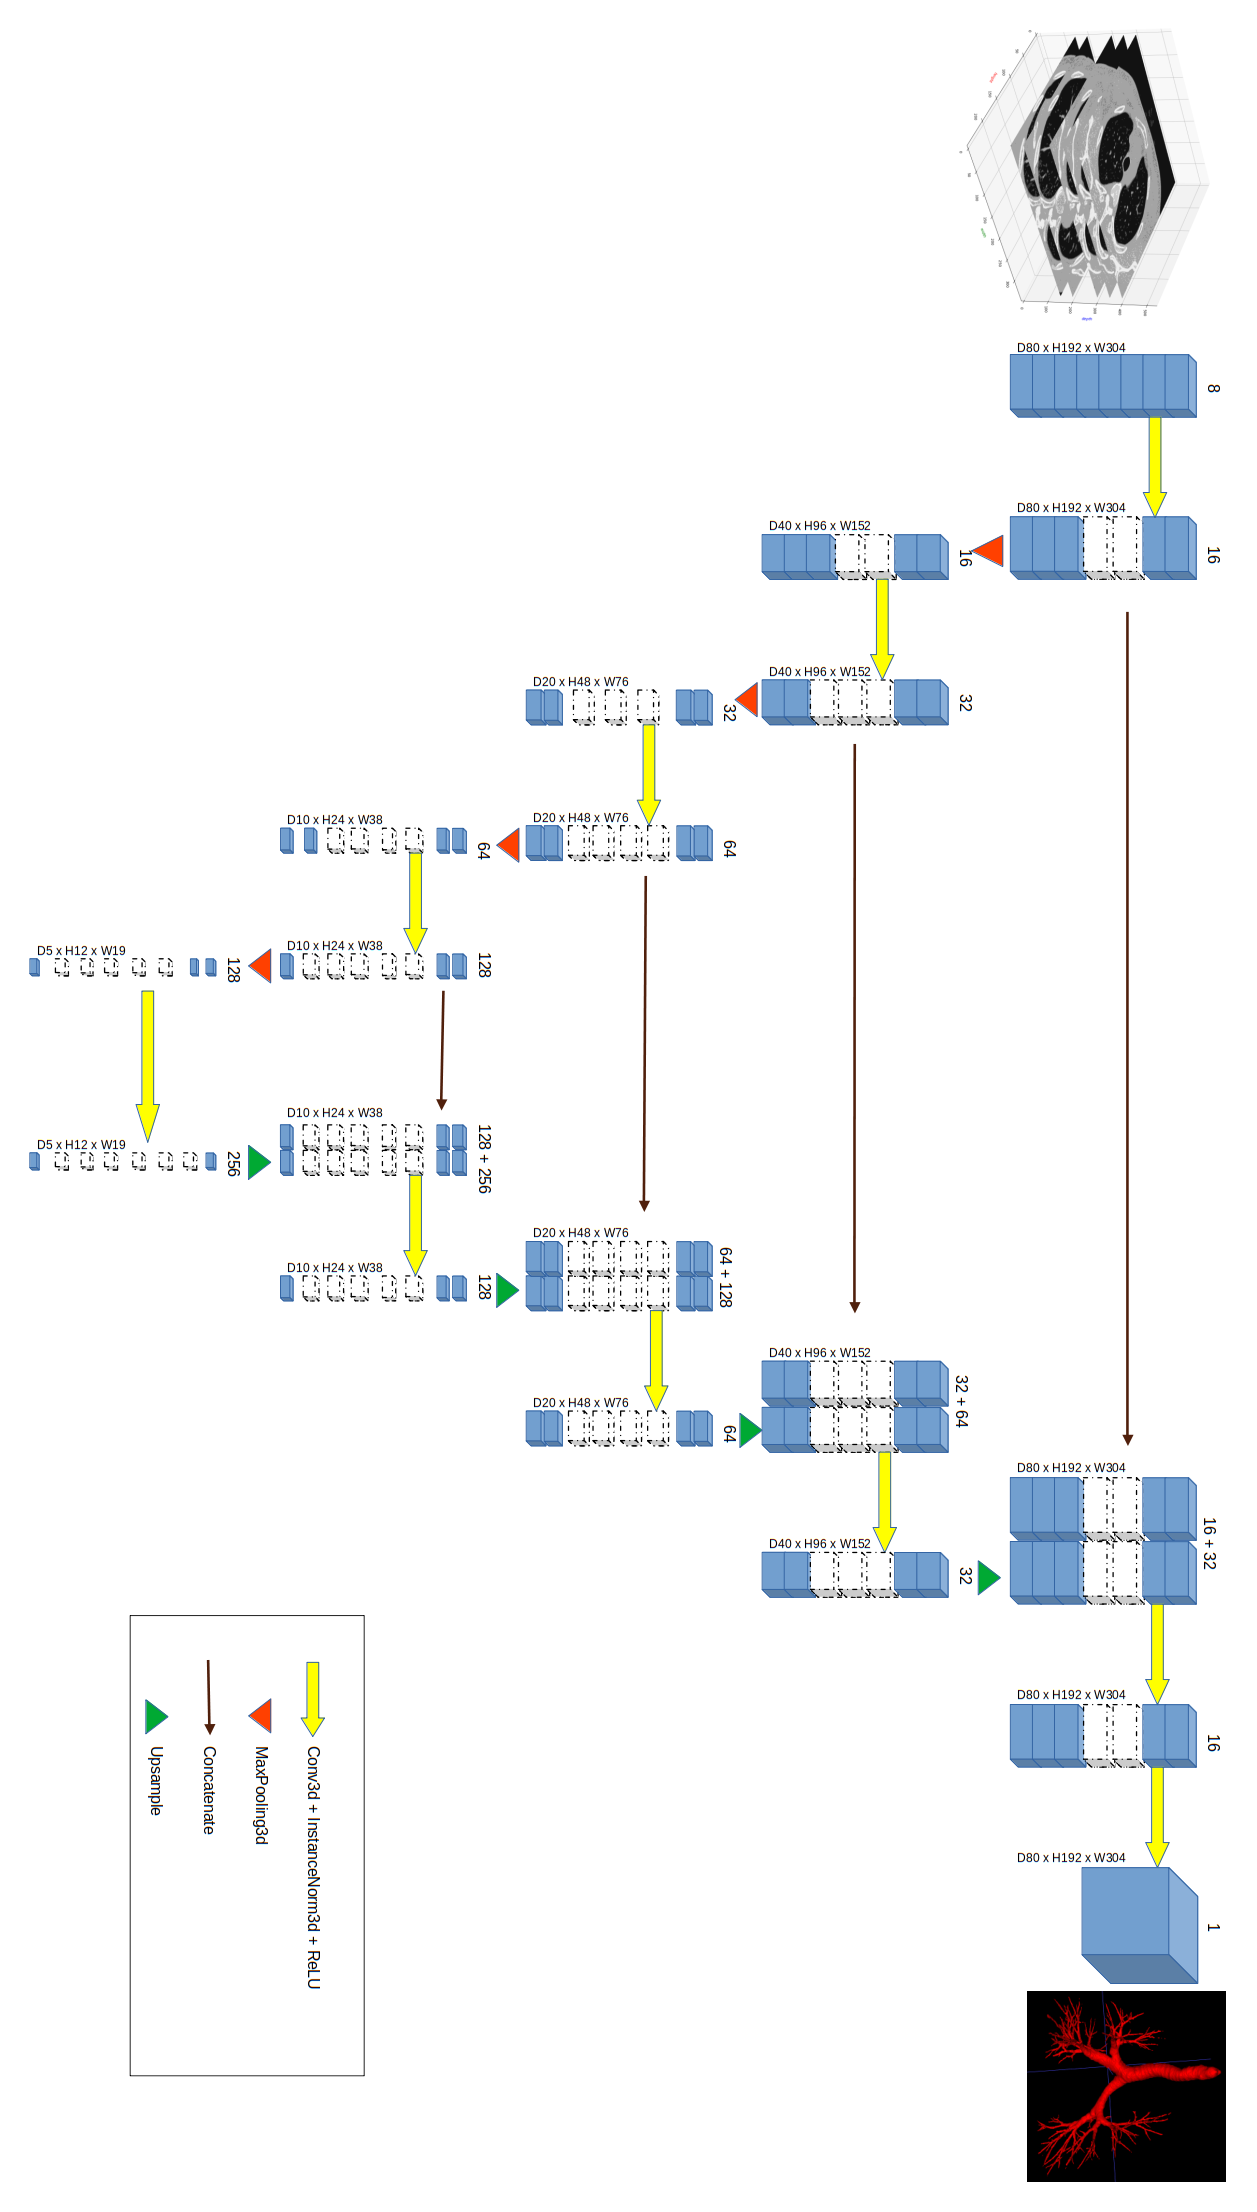
\includegraphics[height=0.72\textheight]{3DUNet_Structure_portrait}
    \bicaption[本文所设计与使用的3D-UNet网络结构]
        {本文所设计与使用的3D-UNet网络结构}
        {The 3D-UNet structure we designed in this paper}
    \label{fig:3DUNetStructure}
\end{figure}
送入网络之前,我们将其裁切为一个一个$D80 \times H192 \times W304$规格的长方体\footnote{我们将在后文讲述为什么裁切
成$D80 \times H192 \times W304$规格的。},网络学习长方体的图像特征,分割长方体内的支气管分支。训练完成后我们将属于同
一个原始CT图像的所有长方体拼接起来,最终分割出来完整的支气管气道树(网络右侧)。在长方体上面标出来的数字表示经过卷积操作后输出
的特征通道数,而在长方体侧面标注的诸如$D20 \times H48 \times W76$表示经过池化后,长方体的体积扩大或缩小,也就是长方体内
体素的分辨率增大或减小。需要指出的是,在U型结构的右侧,每一个层靠近跳跃连接的箭头处都有一个并排的长方体柱,那表示跳跃连接将
下采样路径上每一个卷积层块的特征输出拼接到上采样路径上每一个对应的反卷积层块的输入特征来。

上述的3D-UNet网络结构是本文所设计与使用,并编程实现的CT图像支气管气道树分割网络。我们将以此3D-UNet网络作为基准,通过实验
分析3D-UNet的分割结果和性能指标(包括但不限于假阳性率False Positive Rate、 真阳性率True Positive Rate、骰子相似度
系数Dice Similarity Coefficient、分支检出率Branch Detected、检测到的树长Tree Length Detected和精度等指标),提出
我们的改进方法。我们将在后面的章节展开讲述我们的改进方法,并通过实验来对比验证我们的改进方法是否有效,是否提高了分割效果和性能。

\subsection{损失函数、优化器与学习率调整}
\subsubsection{Dice损失函数}
我们为3D-UNet网络基准模型采用普遍的骰子损失函数Dice Loss, 其计算公式\ref{eq:dice_loss}
\begin{equation}\label{eq:dice_loss}
    L_{dice}\left(Cuboid_{pred}, Cuboid_{gt}\right) = 1 - \frac{2\sum{\left(Cuboid_{pred} \cdot Cuboid_{gt}\right)} + \epsilon}
    {\sum{Cuboid_{pred}} + \sum{Cuboid_{gt}} + \epsilon}
\end{equation}
其中${Cuboid}_{pred}$表示预测值三维矩阵,${Cuboid}_{gt}$表示真实值三维矩阵,此三维矩阵的大小为\ref{sec:ATM22dataset}
节中切割出来的长方体子块的大小$z \times y \times x = 80 \times 192 \times 304$. 而$\epsilon$是为防止除零而加入的平滑常数,
$Cuboid_{pred} \cdot Cuboid_{gt}$表示这2个三维矩阵的点积。

\subsubsection{Adam优化器与动态调整学习率}
支气管气道树分割是属于数据分布稀疏的场景,即有效的支气管体素在整个CT体素中的占比非常小,我们可以从ATM22数据集中随机挑选5个
病例,统计支气管体素在整个CT体素的占比来看稀疏程度。
\begin{table}[!htp]
    \bicaption[支气管体素占比]{支气管体素占比}{The percent of bronchus voxels over total voxels}
    \label{tbl:bronchus_voxels}
    \centering
    \begin{tabular}{crrr}
        \toprule
        病例名称 & 支气管体素 & 总体素 & 支气管体素占比 (\%)\\
        \midrule
        ATM\_009\_0000 &	 115,366 &	 209,453,056 &	 0.055 \\
        ATM\_027\_0000 &	 48,503  &	 161,218,560 &	 0.030 \\
        ATM\_016\_0000 &	 182,904 &	 187,170,816 &	 0.097 \\
        ATM\_033\_0000 &	 127,045 &	 171,704,320 &	 0.073 \\
        ATM\_023\_0000 &	 141,790 &	 209,453,056 &	 0.067 \\
        \bottomrule
    \end{tabular}
\end{table}
从表\ref{tbl:bronchus_voxels}可以看出,支气管体素占比都不到$0.1\%$,因此我们弃选随机梯度下降(Stochastic Gradient
Descend, SGD)优化器。为了更好地利用稀疏梯度信息,达到更好地收敛,我们选择Adam优化器。但是对Adam优化器,我们做了一些修改,
采用动态调整学习率。
让我们来看看Adam优化器\cite{Kingma2014AdamAM}计算梯度和更新参数的过程,来解释我们为什么采用动态调整学习率的方法。

\noindent{}网络模型的参数向量$\theta$在$t$时间步
\begin{equation}
\theta_{t} = \begin{bmatrix}
    \theta_{1} \\
    \theta_{2} \\
    \vdots      \\
    \theta_{n}
\end{bmatrix}_{t}
\end{equation}
计算在$t$时间步的梯度$grad_{t}$
\begin{equation}
    {grad}_{t} = \nabla_{t}J(\theta_{t})
\end{equation}
依据梯度的指数移动平均,计算在$t$时间步的一阶矩估计$m_{t}$
\begin{equation}
    m_{t} = \beta_{1} m_{t-1} + (1 - \beta_{1}) {grad}_{t}
\end{equation}
其中$\beta_{1}$为指数衰减率,控制权重分配、动量和当前梯度,默认取0.9。

\noindent{}依据梯度平方的指数移动平均,计算在$t$时间步的二阶矩估计$v_{t}$
\begin{equation}
    v_{t} = \beta_{2} v_{t-1} + (1 - \beta_{2}) {grad}_{t}^{2}
\end{equation}
其中$\beta_{2}$为指数衰减率,控制之前梯度的平方的影响,对梯度的平方进行加权平均,默认取0.999。

\noindent{}由于一阶矩估计$m_{t}$初始化为0,即$m_{0} = 0$,这会导致$m_{t}$偏向于0,特别是在训练早期阶段。为此我们需要对$m_{t}$进行
偏差纠正,降低偏差对训练早期的影响。
\begin{equation}
    \widehat{m_t} = \frac{m_t}{1 - \beta_{1}^{t}}
\end{equation}
其中$\beta_{1}^{t}$表示计算指数衰减率$\beta_{1}$的$t$次幂。

\noindent{}同样地,我们也需要对二阶矩阵估计$v_{t}$进行偏差纠正。
\begin{equation}
    \widehat{v_t} = \frac{v_t}{1 - \beta_{2}^{t}}
\end{equation}
$\beta_{2}^{t}$类似地表示对指数衰减率$\beta_{2}$的$t$次幂。

\noindent{}最后我们来更新在$t$时间步的参数$\theta_{t}$,学习率$lr$乘以梯度均值$\widehat{m_t}$与梯度方差的平方根
$\sqrt{\widehat{v_t}}$之比。为防止除零而引入平滑常数$\epsilon = 1 \times {10}^{-8}$
\begin{equation}\label{eq:adam_update_params}
    \begin{bmatrix}
        \theta_{0} \\
        \theta_{1} \\
        \vdots \\
        \theta_{n}
    \end{bmatrix}_{t} = 
    \begin{bmatrix}
        \theta_{0} \\
        \theta_{1} \\
        \vdots \\
        \theta_{n}
    \end{bmatrix}_{t-1} -
    {lr} * \frac{\widehat{m_t}}{\sqrt{\widehat{v_t}} + \epsilon}
\end{equation}
在式\ref{eq:adam_update_params}中,若分母$\sqrt{\widehat{v_t}}+\epsilon$过小,就会产生过大的参数$\theta_{t}$,
这会导致在接近最优值的“山峰”或“山谷”时会反复振荡,所以我们采取降低学习率的方法来稍微抵消一些。在训练的过程中,我们会逐渐地
动态地降低学习率。具体降低学习率的策略是:如果训练时的损失保持在一个平台超过10个epoch,我们就会降低学习率10倍, 
在训练后期我们会将这个周期拉长为20g个epoch。初始学习率设置为$3 \times {10}^{-3}$,动态降低学习率按照表
\ref{tbl:descend_lr}的规律来进行调整。
\begin{table}[!htp]
    \bicaption[动态降低学习率]{动态降低学习率}{Dynamically descent the learning rate}
    \label{tbl:descend_lr}
    \centering
    \begin{tabular}{cc}
        \toprule
        Epoch \# & Learning rate \\
        \midrule
        1 & $3 \times {10}^{-3}$ \\
        11 & $3 \times {10}^{-4}$ \\
        21 & $3 \times {10}^{-5}$ \\
        41 & $3 \times {10}^{-6}$ \\
        60 & $3 \times {10}^{-6}$ \\
        \bottomrule
    \end{tabular}
\end{table}


\subsection{模型实现和运行环境}
本文的模型是采用Python v3.10.9版本编写的,基于PyTorch v1.13.1框架实现3D-UNet模型的。本文的代码编写调试和模型训练均是
在上海交通大学高性能计算中心提供的AI超算平台上进行的。该AI超算平台由8台DGX-2组成,每台DGX-2配备16块NVIDIA Tesla V100显卡,
深度学习张量计算能力达到16PFLOPS。详细的配置与计算能力如表\ref{tbl:AT_platform}所示:
\begin{table}[!htp]
    \caption{人工智能超算平台资源}
    \label{tbl:AT_platform}
    \centering
    \begin{tabular}{c|l|c}
        \toprule
        队列 & 参数 & 节点数量 \\
        \midrule
        dgx2 & CPU: 2*Intel Xeon Scalable Cascade Lake 8168 (2.7GHz, 24 cores) & 8 (16卡/节点) \\
             & Memory: 1.5TB DDR4 ECC REG 2666 & \\
             & GPU: 16*NVIDIA Tesla V100 & \\
        \bottomrule
    \end{tabular}
\end{table}
本文的实验被分配最多8块显卡,由于有多个对比实验同时运行,因此不是8块显卡被一个实验独占使用。一般地我为轻计算量的实验分配2块
显卡,为重计算量的实验分配4块显卡。这样在同一个时间段就可以同时执行多个计算任务,使对比实验可以并行进行。

由于本文的实验是在超级计算机上执行,完全不同于传统的普通台式机、工作站等环境,因此有必要讲解清楚本文的实验运行环境。AI超算平台
使用Slurm作业调度系统(如图\ref{fig:slurm_job_system})来执行超算用户提交的计算任务,用户需要编写专有的Slurm作业脚本来提交作业请求。
\begin{figure}[!htp]
    \centering
    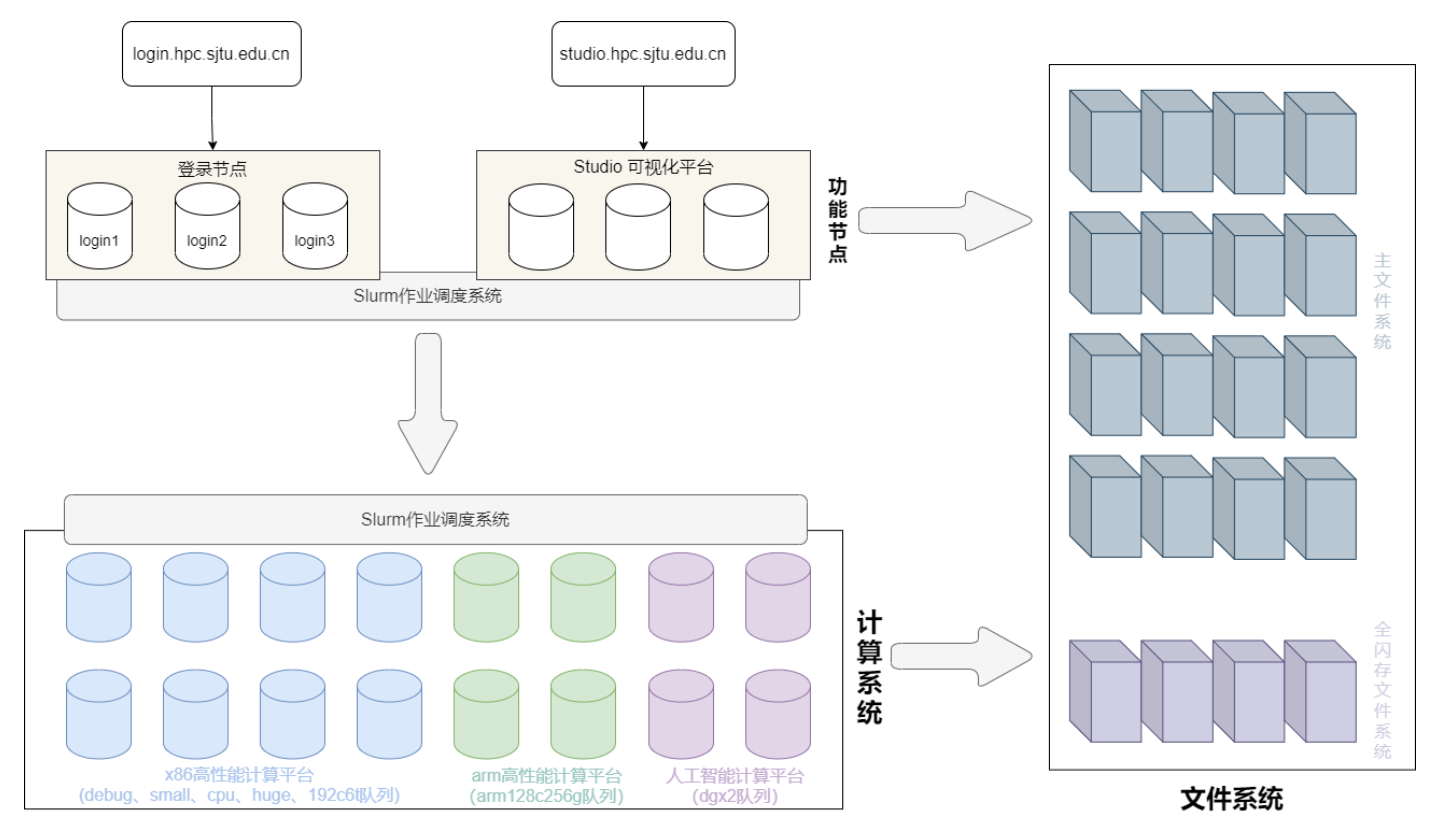
\includegraphics[width=0.8\textwidth]{Supercomputer_Slurm_Job_system}
    \bicaption[AI超算平台Slurm作业调度系统]
        {AI超算平台Slurm作业调度系统\parencite{HpcSlurm2022}}
        {The Slurm job scheduling system on AI supercomputer platform}
    \label{fig:slurm_job_system}
\end{figure}
Slurm脚本里指定当前作业需要用到的CPU核数,需要用到多少张GPU显卡,多少个进程,占用多少个计算节点。这是大规模并行计算需要指定
的计算资源。除此之外,还要配置Python-PyTorch环境,用户准备好可执行程序启动方式,设置好参数选项。最后通过 
\$sbatch Airway3DSegment\_Baseline.slurm命令提交作业,Slurm作业调度系统分配好计算资源后才开始执行计算任务。

\section{数据集ATM22}\label{sec:ATM22dataset}\label{sec:ATM22}
本文使用的数据集是公开的ATM22数据集\cite{Zhang2022CFDA, Zhang2021Airway, Yu2022Bronchi, Qin2019AirwayNet},
是由上海交通大学医疗机器人研究院联合上海胸科医院从多家医疗机构,多台不同品牌型号的CT扫描仪收集500例就诊者的胸腔扫描图像,然后
由三名具有五年以上专业经验的放射科医生对气道树结构进行精细的标注。ATM22数据集融合了EXACT'09数据集和LIDC-IDRI部分病例
的数据。我们随机选取了66例CT扫描图像作为训练集, 9例作为验证集,19例作为测试集。训练集、验证集和测试集的比例基本按照70:10:20
的比例来。由于ATM22数据集是采自不同医疗机构、不同品牌型号的CT扫描仪,因此我们对数据进行了预处理,将这些CT图像的体素强度统一截断
在$[-1000, 400]$亨式单位Hounsfield unit的窗口范围内,并归一化到$[0, 1]$范围。

ATM22数据集里的CT图像切片的尺寸基本都是H512 $\times$ W512个像素,存在很大面积的黑色背景,为了避免学习到肺部之外的无关
区域,我们对其进行裁切,只保留肺的最小包围框作为有效的区域,“喂给”深度网络进行学习。裁切前后的肺部区域效果对比如图
\ref{fig:cropimage}所示,
\begin{figure}[htbp]
    \centering
    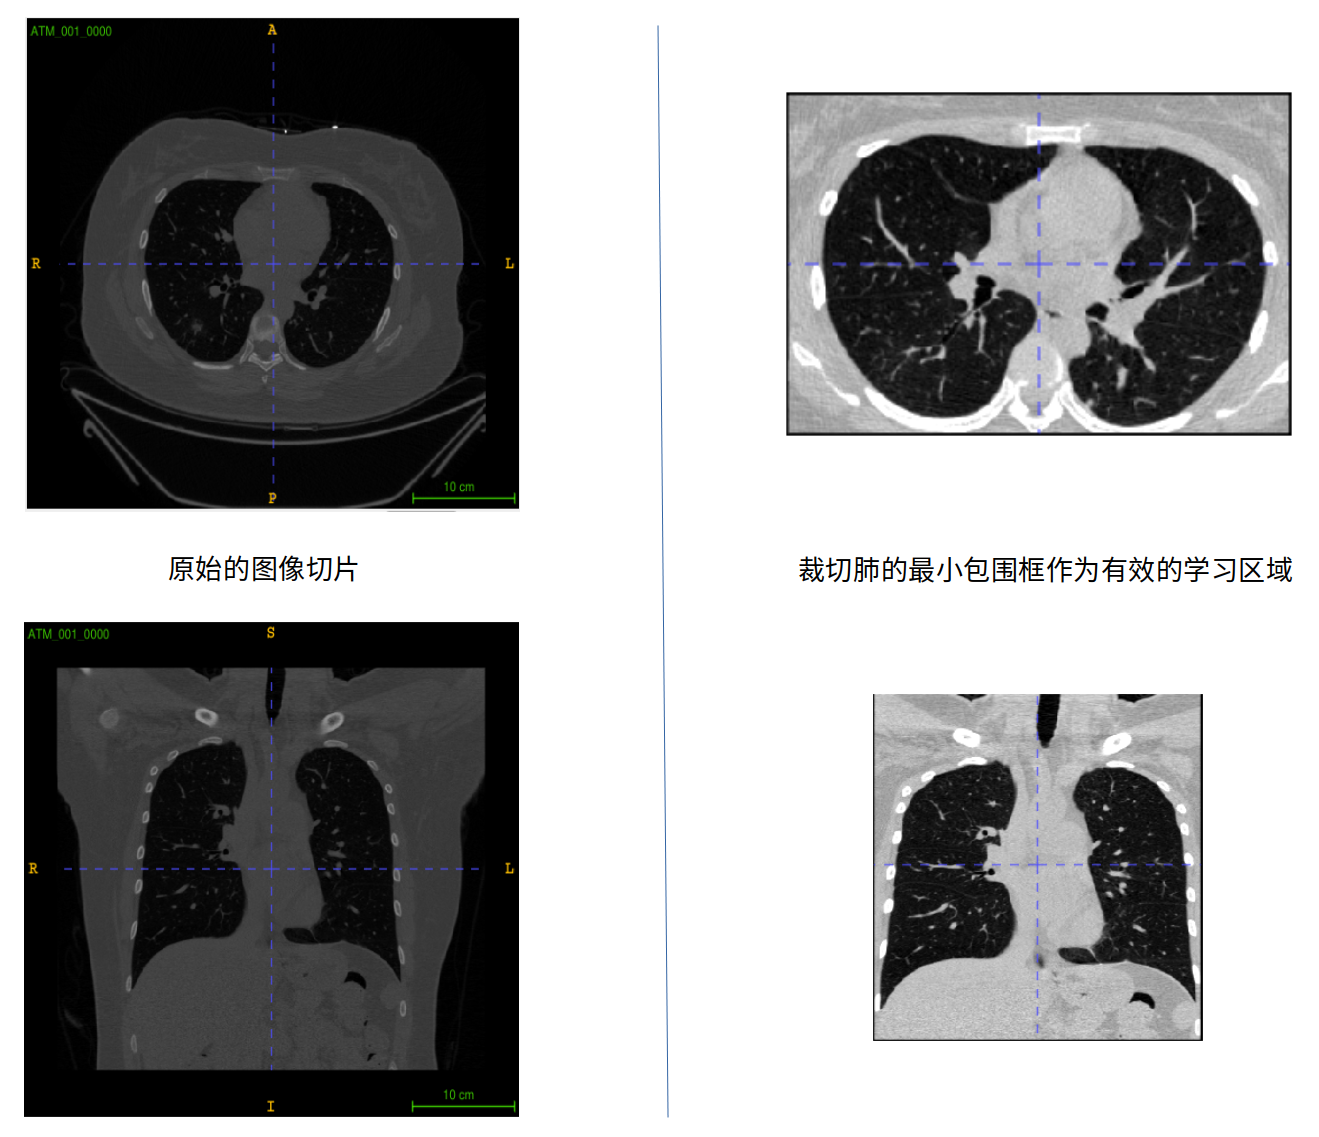
\includegraphics[width=0.7\textwidth]{image_crop}
    \caption{裁切CT图像切片的效果对比}
    \label{fig:cropimage}
\end{figure}
裁切后不仅可以减少计算量,最重要的是排除无关区域对网络的权重与偏置参数产生影响。

经过上述的裁切后,CT图像体的体积大幅缩小,就拿图\ref{fig:cropimage}的ATM-001-0000病例来说,CT图像体从
$D679 \times H512 \times W512$缩减到$D595 \times H225 \times W333$。但即使如此,对于单个GPU单元显存来说仍然比较大,
为此,我们将CT图像体切割成$D80 \times H192 \times W304$尺寸的长方体子块。本文使用由上海交通大学高性能计算中心提供的AI超算平台
来进行训练与计算的。AI超算的显卡型号为NVIDIA Tesla V100,切割成这样的长方体子块最大化利用了GPU的资源又不至于撑爆,可以
允许调整Batch size。本文的网络在训练时分别使用了1/2/4/8四种不同的Batch size, 经测试验证$D80 \times H192 \times W304$
的长方体子块在GPU显存中均运行良好。我们对训练集、验证集和测试集的CT图像体采用了如此相同的切割方法和尺寸。当然,你可能根据你的
GPU显存资源决定切割的长方体子块的大小,显存资源比较大则可以选择切割成更大的长方体子块。我们对CT图像体采用滑动窗口的切割方式,
在训练阶段滑动窗口的大小为$D64 \times H96 \times W152$,在验证和测试阶段则的滑动窗口大小为$D64 \times H72 \times W72$.
滑动窗口的意思是每次切割之前沿着宽度W、高度H、深度D方向逐次移动指定的距离。

为了增强训练效果,也是为了大幅扩大数据量,我们对每个切割的长方体子块图像块进行了数据增强,具体的数据增强方式有:
\begin{enumerate}\label{enum:data_augmentation}
    \item {\heiti 沿深度、高度、宽度三个轴随机翻转 RandomFlip}
    \item {\heiti 随机仿射变换并重采样 RandomAffine}
    \item {\heiti 随机高斯滤镜模糊图像 RandomBlur}
    \item {\heiti 给图像添加随机高斯噪声 RandomNoise}
    \item {\heiti 随机运动模糊,使图像产生运动伪影 RandomMotion}
    \item {\heiti 添加随机偏差场伪影 RandomBiasField}
    \item {\heiti 添加随机spike伪影,在图像空间产生不同方向的条纹 RandomSpike}
    \item {\heiti 添加随机残影 RandomGhosting}
\end{enumerate}
以上数据增强方式,我们通过组合不同的增强方式来联合增强切割的长方体子块图像数据。我们还加入随机概率作用于这些数据增强方式,
进一步增强图像数据。


\section{评价指标和分割效果可视化}
对于支气管气道树的分割任务,其目标是分割出精确的支气管三维模型,用于临床辅助诊疗。评价支气管气道树分割质量的好坏,有如下指标:
\begin{enumerate}
    \item 假阳性率 False Positive Rate, FPR
    
    假阳性代表着误检,也就是说将本不是支气管的体素错误地判定为支气管体素。假阳性率越高表示错误检查发生越多,分割结果愈不可信。
    
    \item 假阴性率 False Negative Rate, FNR
    
    假阴性代表着漏检,就是将本来是真实的支气管体素漏掉了,而认为是普通的背景体素。假阴性过高会导致临床诊断时可能将潜藏的真实
    疾病漏诊,而贻误了治疗时机。
    
    \item 灵敏度 Sensitivity
    
    灵敏度也叫真阳性率(True Positive Rate, TPR),其表示检测出来的真实支气管体素占实际的全部支气管体素的比例。 
    
    \item 精度 Precision
    
    精度表示检测出来的真实支气管体素跟真实的支气管体素与发生误检的假阳性支气管体素之和的比例,精度代表着模型的分割能力。在
    95\%的置信区间内,模型能辨识出实际的真实支气管体素的能力。精度越高,表示分割出来的支气管气道树越接近患者的真实情况,就能
    更可靠地帮助临床医生做出准确的病情诊断。
    
    \item 骰子相似度系数 Dice Similarity Coefficient, DSC
    
    DSC用来衡量网络分割的结果与金标准之间的相似性,是一种集合相似度度量函数。表示为预测的支气管体素与真实的支气管体素的交集
    跟预测的支气管体素加上真实的支气管体素进行比较。
    
    \item 检测到的分支 Branch Detected, BD
    
    BD表示模型检测到的分支数相比于参考的实际存在的分支总数
    
    \item 检测到的树长 Tree Length Detected, TLD
    
    树长为模型检测到的所有分支的中心线长度之和,TLD表示检测到的树长相比于参考的真实的树长。
\end{enumerate}
上述这些评价指标是在EXACT'09\cite{Lo2012ExtractionOA}上被提出,并被普遍接受和广泛使用的评价指标。评估的重点是放在提取
最完整的气道树,进入更高代的气道\footnote{注:在医学上通常使用代来表示支气管分支的相对关系。从咽喉部一直到肺部气管第一个分岔
前的气管称为第0代气管,从第一个分岔出来的左右肺主气管称为第1代气管,然后分岔到上/中/下肺叶的气管称为第2代气管,再分岔到段支气管
的称为第3代气管。如此类推,每分岔一个支气管,气管的代就增加1。气管的代越高,表示气管管腔直径就越细小。}并提取尽可能多的分支。

如何计算这些评价指标,我们以模型预测的支气管体素对比真实的支气管体素的比对表\ref{tbl:metrics_calculation}来说明,
并定义计算方法。
\begin{table}[!htp]
    \bicaption[评价指标计算方法说明]{评价指标计算方法说明}{The explanation of metrics calculation}
    \label{tbl:metrics_calculation}
    \centering
    \begin{tabular}{c|c|c|c|c}
        \hline
        \makecell{模型预测的支\\气管体素} & \makecell{真实的支气\\管体素} & \makecell{表示}  & 体素个数 
        & \makecell{在ITK-SNAP中\cite{Yushkevich2006ITKSNAP}的\\颜色标记} \\
        \hline
        1  &  0  & 假阳性 & ${Voxel}_{FP}$ & \textcolor{green}{绿色} \\
        \hline
        1  &  1  & 真阳性 & ${Voxel}_{TP}$ & \textcolor{blue}{蓝色} \\
        \hline
        0  &  0  & 真阴性 & ${Voxel}_{TN}$ & \textcolor{black}{黑色(背景)} \\
        \hline
        0  &  1  & 假阴性 & ${Voxel}_{FN}$ & \textcolor{red}{红色} \\
        \hline
    \end{tabular}
\end{table}
依据表\ref{tbl:metrics_calculation},上述的指标按如下的公式计算:
\begin{enumerate}
    \item 假阳性率
    
    \begin{equation}
        FPR = \frac{{Voxel}_{FP}}{{Voxel}_{FP} + {Voxel}_{TN}} \times 100\%
    \end{equation}
    
    \item 假阴性率
    
    \begin{equation}
        FNR = \frac{{Voxel}_{FN}}{{Voxel}_{FN} + {Voxel}_{TP}} \times 100\%
    \end{equation}
    
    \item 灵敏度
    
    \begin{equation}
        Sensitivity = \frac{{Voxel}_{TP}}{{Voxel}_{TP} + {Voxel}_{FN}} \times 100\%
    \end{equation}
    
    \item 精度
    
    \begin{equation}
        Precision = \frac{{Voxel}_{TP}}{{Voxel}_{TP} + {Voxel}_{FP}} \times 100\%
    \end{equation}
    
    \item 骰子相似度系数
    
    \begin{equation}
        DSC = \frac{2 * {Voxel}_{TP}}{({Voxel}_{TP} + {Voxel}_{FN}) + ({Voxel}_{TP} + {Voxel}_{FP})} \times 100\%
    \end{equation}
    
    \item 检测到的分支
    
    \begin{equation}
        BD = \frac{{Branch}_{seg}}{{Branch}_{gt}} \times 100\%
    \end{equation}
    其中${Branch}_{seg}$表示分割结果中检测到的分支数, ${Branch}_{gt}$表示真实存在的分支总数
    
    \item 检测到的树长
    
    \begin{equation}
        TLD = \frac{{Len}_{seg}}{{Len}_{gt}} \times 100\%
    \end{equation}
    其中${Len}_{seg}$表示分割结果中检测到的所有分支的中心线长度之和,${Len}_{gt}$表示真实存在的所有分支的中心线长度之和。
\end{enumerate}

经过模型训练后分割出来的支气管气道树,我们可以将其导入到ITK-SNAP\cite{Yushkevich2006ITKSNAP}软件中显示分割效果。这里
我们选择ATM\_054\_0000这个病例来可视化支气管气道树分割3D模型(这是经过3D-UNet基准网络分割的结果),如图
\ref{fig:airway_tree_model}所示。
\begin{figure}[!htp]
    \centering
    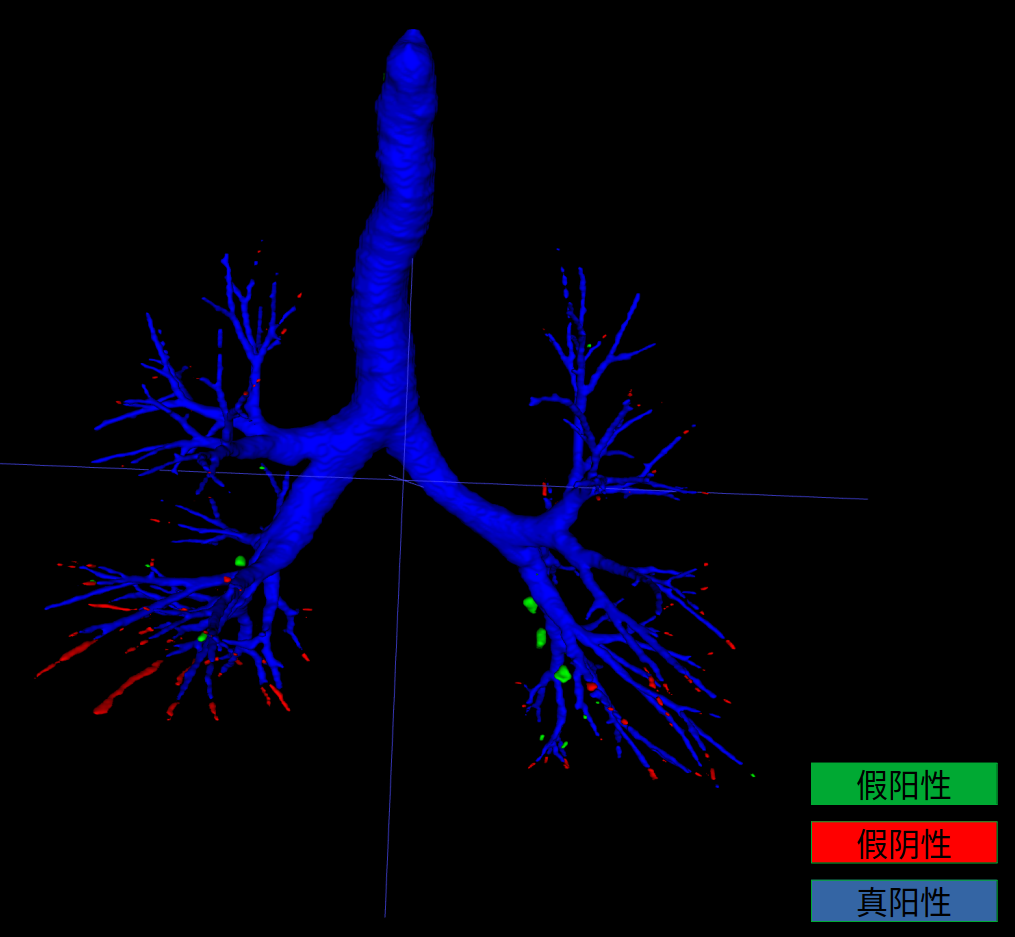
\includegraphics[width=0.8\textwidth]{visualize_colored_airway_tree}
    \bicaption[支气管气道树分割的3D模型]
        {支气管气道树分割的3D模型}
        {The 3D model of airway tree after segmentation}
    \label{fig:airway_tree_model}
\end{figure}
图例中\textcolor{green}{绿色}的表示\textcolor{green}{假阳性}体素,\textcolor{red}{红色}的表示\textcolor{red}{假阴性}
体素,\textcolor{blue}{蓝色}的表示\textcolor{blue}{真阳性}体素。

假阳性体素说明分割模型发生了误检,从图\ref{fig:airway_tree_model}可以明显看出绿色的体素跟气道树枝杆是分离的,不属于支气管
体素,而应该是黑色的背景体素,但3D-UNet分割模型却错误地认为是支气管体素。 假阴性说明分割模型发生了漏检,红色的体素原本是真实
存在的支气管,但3D-UNet分割模型漏掉了这些真实存在的支气管体素。这些漏掉的真实存在的支气管体素都是在支气管气道树的末端,是
属于非常细小的支气管,3D-UNet分割模型没有把这些细小的支气管体素分割出来,说明分割模型的能力还不够精细。最后,蓝色的体素则是
表明分割模型分割出来的支气管体素与真实存在的支气管体素是完全吻合的。粗大的气管、左右肺主支气管、上/中/下肺叶支气管和较细的段
支气管都被正确地分割出来,但在更细小的小叶支气管分割能力方面则显得还不够。

需要指出的,本中文对支气管气道树分割的颜色标记统一为绿色表示假阳性,红色表示假阴性,蓝色表示真阳性。全文保持一致的颜色标记,
后文中若没有特别指出颜色标记的意义,均视为与此处一致,不再重复地给出图例说明。

\section{实验结果与分析}
\subsection{3D-UNet基准网络训练过程}
我们将3D-UNet基准网络放在上海交通大学高性能计算中心的AI超级计算机上进行训练,输入是从ATM22数据集上随机挑选66例肺部CT扫描图像,按照
\ref{sec:ATM22}节介绍的裁切方法去掉无关的黑色背景区域,只保留肺部最小包围框作为有效学习区域。然后将这些经裁切的Cuboid体数据
按照$D64 \times H96 \times W152$的滑动窗口步长随机切割成$D80 \times H192 \times W304$的子块,每个子块都经过
\ref{enum:data_augmentation}节所述的8种数据增强方法进行增强。Label数据也是66例同病例的CT体数据,按照同样的方式进行
裁切和切割成$D80 \times H192 \times W304$的子块,但这些Label子块不进行数据增强。每一个图像Cuboid体数据子块与对应的
Label体数据子块绑定在一起。训练集、验证集和测试集的CT图像切割情况如表\ref{tbl:dataset_overview}所示。
\begin{table}[!htp]
    \bicaption[训练集、验证集和测试集的数据一览]{训练集、验证集和测试集的数据一览}
        {Overview of the cropped CT cube images among trainset, validateset and testset}
    \label{tbl:dataset_overview}
    \centering
    \begin{tabular}{c|c|c}
        \toprule
          & \makecell{CT扫描图像\\例数} & \makecell{切割成$D80 \times H192 \times W304$\\的子块总数} \\
        \midrule
        训练集 & 66 & 2202 \\
        验证集 & 9  & 415 \\
        测试集 & 19 & 770 \\
        \bottomrule 
    \end{tabular}
\end{table}
我们还会在将这些子块送给网络进行学习前会进行一次洗牌,完全打乱2202个子块的顺序,每一个迭代周期都会洗牌一次。同样地,我们也对
验证集的415个子块和测试集的770个子块在每个迭代周期都进行洗牌。

在训练过程中,我们使用TensorBoard收集每一个迭代周期Epoch的损失函数值,我们密切注视着损失函数的曲线。
我们观察到40多个迭代周期后,损失函数曲线已经平缓了,趋于收敛了,在60个迭代周期后我们便结束了训练过程。训练过程中的损失函数
曲线如图\ref{fig:lossfn_curve}所示。
\begin{figure}[!htp]
    \centering
    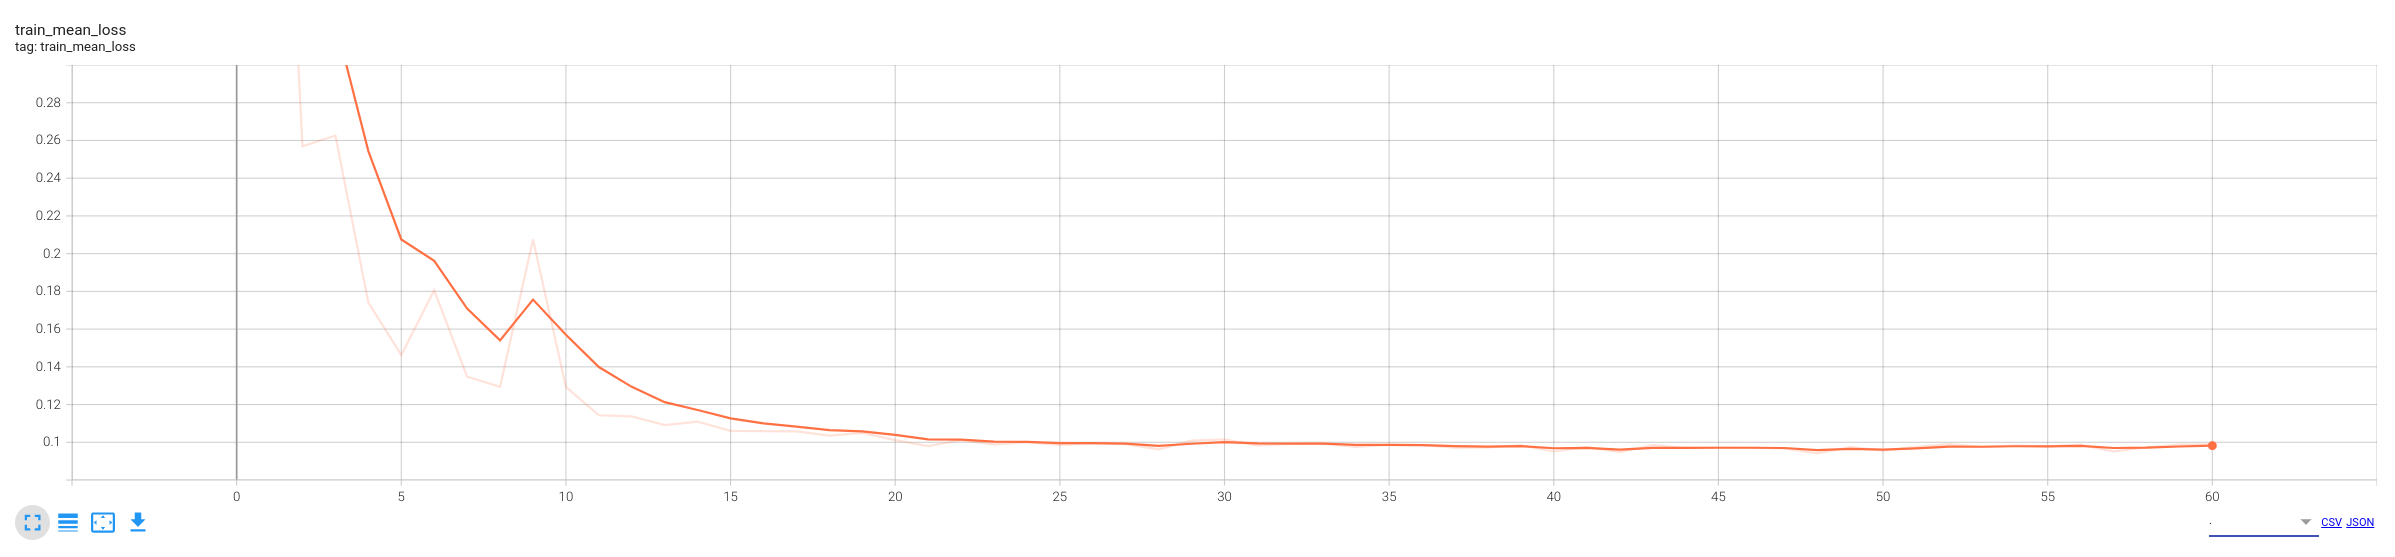
\includegraphics[width=\textwidth]{train_mean_loss_curve}
    \bicaption[3D-UNet基准网络训练时的损失函数曲线]
        {3D-UNet基准网络训练时的损失函数曲线}
        {The loss function curve of 3D-UNet baseline network during training process}
    \label{fig:lossfn_curve}
\end{figure}
在训练过程中,第一个迭代周期我们就对验证集的9例CT图像进行分割,输出每例CT图像的支气管气道树3D模型和指标数据。当然这个分割结果
肯定是非常糟糕的,但我们将它视为检验程序正确运行的参照物,训练迈出第一步的标志。之后每经过10个迭代周期,程序就会对验证集和测试集
里的CT图像进行分割,输出并保存每例CT图像的支气管气道树3D模型和指标数据。每5个迭代周期都会保存模型的Check Point状态和参数,
并以model\_epochnum.ckpt文件名(如第35个迭代周期的模型名字就是model\_035.ckpt)格式保存下来。这样可使我们能够在训练中断后
沿着上次的model\_xxx.ckpt继续训练,而不用浪费时间从头开始训练。训练完成后将模型Check Point状态和参数保存为model\_latest.ckpt,
作为后续验证过程和测试过程的预训练模型,直接加以使用。除了保存模型Check Point状态后参数外,我们在每10个迭代周期将指标数据
保存进TensorBoard。累积这些数据帮助我们观察网络的优化发展状况,分析这些数据帮助我们找到改进方向。

在验证过程中,我们直接使用预训练模型model\_latest.ckpt对验证集里的9例CT图像进行分割,输出每例CT图像的支气管气道树3D模型
和指标数据。在测试过程中,我们对测试集里的19例CT图像执行同样的操作。我们将在\ref{subsec:experiment_results}节展示这些
实验结果。

以上的训练、验证和测试过程均在一次提交的Slurm作业里完成。 3D-UNet基准网络使用了2张NVIDIA Tesla V100显卡,Batch-size
设置为4,即一次读入4个$D80 \times H192 \times W304$的子块,2202个子块需要551次循环才能算完,启动4个进程进行并行计算。
训练过程每个迭代周期平均耗时658.7秒,验证过程跟训练过程同样的设置,每迭代周期平均耗时4137.6秒,而测试过程每迭代周期平均耗时9309.6秒。
详细的运行时间见表\ref{tbl:time_consumption}。为什么每迭代周期验证耗时和测试耗时都明显比训练耗时要长得多? 这里需要解释一下。
验证过程需要对9例CT图像计算评价指标数据,还需要计算产生三维气道树模型。每计算一个三维气道树模型需要耗时6分钟之久,计算BD和TLD两个
指标也需要耗时5分钟左右。重要的是,计算三维气道树模型和BD、TLD指标数据无法使用GPU进行并行计算而加速,只能采用CPU串行计算方式。
这主要是三维气道树模型和BD、TLD指标的计算涉及到很多的逻辑判断,加之Python Numpy库函数没有GPU版本的,所以无法使用GPU加速计算。
\begin{table}[ht]
    \centering
    \bicaption[3D-UNet基准网络训练、验证、测试耗时一览表]
        {3D-UNet基准网络训练、验证、测试耗时一览表}
        {Time consumption of training, validating and testing on 3D-UNet baseline}
    \label{tbl:time_consumption}
    \scalebox{0.8}{
    \begin{tabular}{c|c|c|c||c|c|c|c}
        \hline
        \multicolumn{8}{c}{运行时间 (单位: 秒)} \\
        \hline
        \makecell{迭代\\周期} & \makecell{训练\\耗时} & \makecell{验证\\耗时} & \makecell{测试\\耗时} &
        \makecell{迭代\\周期} & \makecell{训练\\耗时} & \makecell{验证\\耗时} & \makecell{测试\\耗时} \\
        \hline
        1	& 745.56	& 5034.34	&          &   31	& 653.84	&           &         \\
        2	& 656.85	&           &          &   32	& 656.55	&           &         \\            	
        3	& 657.74	&           &          &   33	& 655.44	&           &         \\            	
        4	& 657.58	&           &          &   34	& 655.85	&           &         \\            	
        5	& 657.91	&           &          &   35	& 655.63	&           &         \\            	
        6	& 657.84	&           &          &   36	& 655.75	&           &         \\            	
        7	& 657.86	&           &          &   37	& 656.22	&           &         \\            	
        8	& 657.01	&           &          &   38	& 657.3		&           &         \\            	
        9	& 656.64	&           &          &   39	& 656.49	&           &         \\            	
        10	& 656.53	& 5068.17	& 9560.42  &   40	& 656.66	& 3770.93	& 9457.15 \\
        \hline
        11	& 663.29	&           &          &   41	& 654.77	&           &         \\             	
        12	& 656.7		&           &          &   42	& 656.61	&           &         \\             
        13	& 657.82	&           &          &   43	& 656.63	&           &         \\             	
        14	& 658.24	&           &          &   44	& 656.56	&           &         \\             	
        15	& 658.56	&           &          &   45	& 656.46	&           &         \\             	
        16	& 657.96	&           &          &   46	& 656.78	&           &         \\             	
        17	& 658.15	&           &          &   47	& 656.46	&           &         \\             	
        18	& 657.97	&           &          &   48	& 656.14	&           &         \\             	
        19	& 658.68	&           &          &   49	& 655.84	&           &         \\             	
        20	& 658.03	& 3770.34	& 9557.97  &   50	& 655.97	& 3770.28	& 8337.74 \\ 
        \hline
        21	& 660.52	&           &          &   51	& 656.05	&           &         \\  	
        22	& 656.01	&           &          &   52	& 655.59	&           &         \\  	
        23	& 656.75	&           &          &   53	& 655.69	&           &         \\  	
        24	& 655.99	&           &          &   54	& 656.75	&           &         \\  	
        25	& 656.48	&           &          &   55	& 657.62	&           &         \\  	
        26	& 659.39	&           &          &   56	& 657.26	&           &         \\  	
        27	& 658.22	&           &          &   57	& 658.17	&           &         \\  	
        28	& 659.65	&           &          &   58	& 658.94	&           &         \\  	
        29	& 658.81	&           &          &   59	& 657.99	&           &         \\  	
        30	& 658.45	& 3780.8	& 9544.24  &   60	& 658.28	& 3768.32	& 9399.98 \\ 	 	 	 	 	 	 	  	 	 	 	 	 	 	 	 	 	 	 	 	 	 	 	 	 	 	
        \hline
        61	&	        & 5252.09	&          &   62   &           &           & 9726.56 \\
        \hline
        \hline
        平均 & 658.7     & 4137.6    & 9309.6   & \multicolumn{2}{|c|}{总耗时} & \multicolumn{2}{|c}{38小时50分} \\
        \hline
    \end{tabular}
    }
\end{table}
验证集有9例CT图像,测试集有19例CT图像都需要计算指标数据和产生三维支气管气道树模型,所以每个迭代周期测试集计算耗时是验证集计算耗时
2倍多。 但好在我们不是每个迭代周期都会去计算验证集和测试集,而是每隔10个迭代周期才去计算一次。验证集在第一个迭代周期被计算一次,而
测试集并没有被计算。

表\ref{tbl:time_consumption}反映了我们的整个实验过程。经历了60个迭代周期训练过程完成。在第61个迭代周期,我们使用训练获得的最新模型
参数(即加载最新的预训练模型model\_latest.ckpt)来执行验证过程,第62个迭代周期执行测试过程。最后,3D-UNet基准网络训练、验证和测试全过程
总耗时38小时50分钟,完成一个完整实验。

\subsection{实验结果和分析}\label{subsec:experiment_results}
上述的训练、验证和测试过程完成后,我们来展示实验结果。由于篇幅的原因,我们挑选验证集里的9例CT图像,展示支气管气道树3D模型的
可视化效果和他们的指标数据。而对于测试集里的19例CT图像,19张支气管气道树3D模型图片实在太多放不下,我们只展示19组指标数据。

我们将进行横向和纵向的对比。
\begin{enumerate}
    \item[A.] 在横向对比时,我们对验证集的9例CT图像,每例CT图像均匀地取5张切片,选取中间的那张切片。排列这9张
切片看看它们的分割效果和指标数据,如表\ref{tbl:hcomparison_metrics}所示。

    \begin{table}[!htp]
        \bicaption[验证集CT切片图像分割效果与指标横向比较]
            {验证集CT切片图像分割效果与指标横向比较}
            {Horizontal comparison of segmentation and metrics in the validateset}
        \label{tbl:hcomparison_metrics}
        \centering
        \begin{tabular}{|c|c|c|}
            \hline
            ATM\_029\_0000 & ATM\_054\_0000 & ATM\_055\_0000 \\
            Slice \#296 & Slice \#264 & Slice \#229 \\
            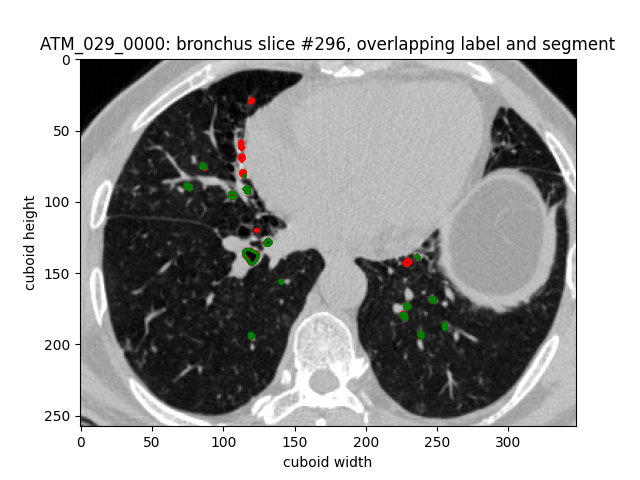
\includegraphics[width=0.3\textwidth]{results/baseline/val060/ATM_029_0000_bronchus_segmentation_slice296_at_val_epoch60} &
            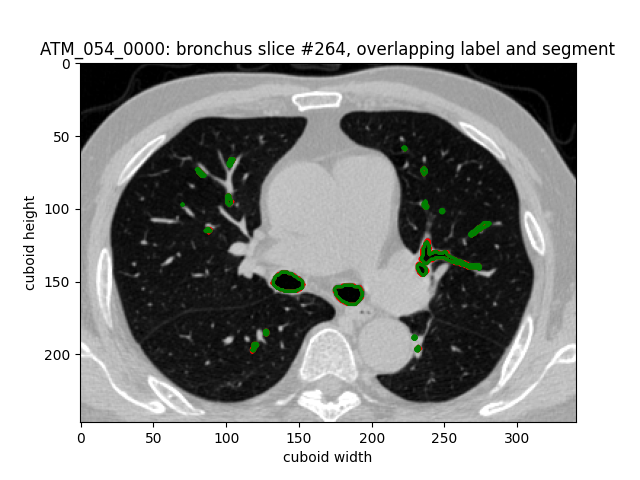
\includegraphics[width=0.3\textwidth]{results/baseline/val060/ATM_054_0000_bronchus_segmentation_slice264_at_val_epoch60} &
            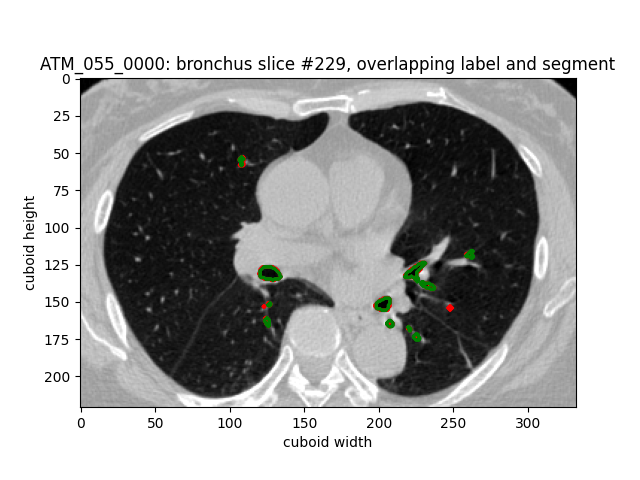
\includegraphics[width=0.3\textwidth]{results/baseline/val060/ATM_055_0000_bronchus_segmentation_slice229_at_val_epoch60} \\
            FPR = 0.066\%           & FPR = 0.068\%             & FPR = 0.056\% \\
            FNR = 14.286\%          & FNR = 5.991\%             & FNR = 9.966\% \\
            Sensitivity = 85.714\%  & Sensitivity = 94.009\%    & Sensitivity = 90.034\% \\
            Precision = 72.558\%    & Precision = 92.039\%      & Precision = 86.469\% \\
            DSC = 78.59\%           & DSC = 93.01\%             & DSC = 88.22\% \\
            \hline
            
            ATM\_057\_0000 & ATM\_091\_0000 & ATM\_174\_0000 \\
            Slice \#287 & Slice \#281 & Slice \#74 \\
            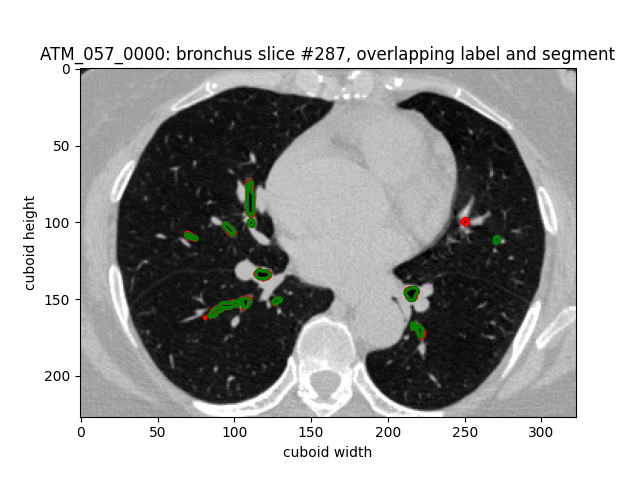
\includegraphics[width=0.3\textwidth]{results/baseline/val060/ATM_057_0000_bronchus_segmentation_slice287_at_val_epoch60} &
            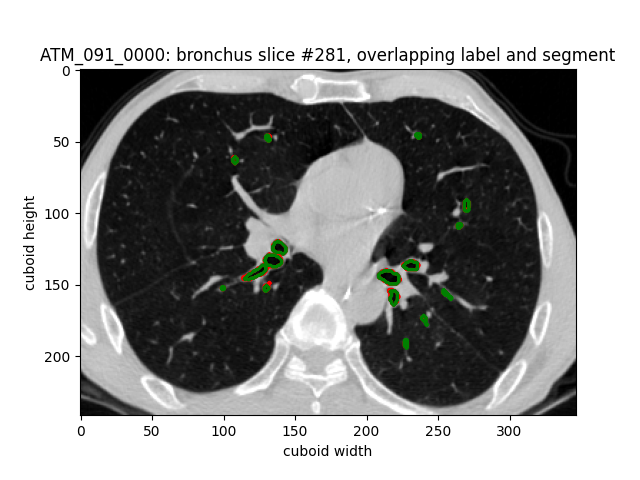
\includegraphics[width=0.3\textwidth]{results/baseline/val060/ATM_091_0000_bronchus_segmentation_slice281_at_val_epoch60} &
            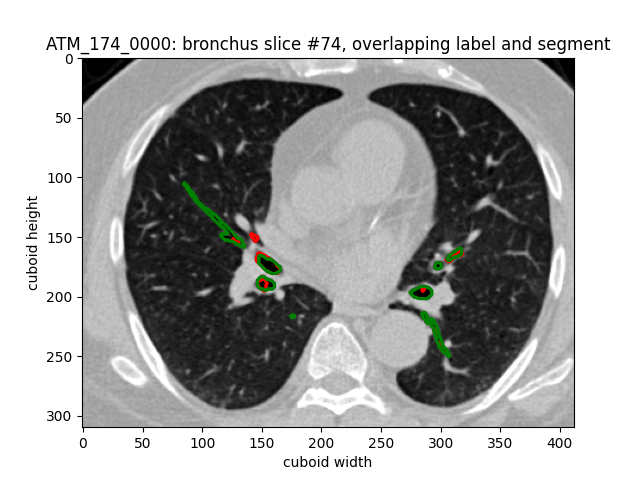
\includegraphics[width=0.3\textwidth]{results/baseline/val060/ATM_174_0000_bronchus_segmentation_slice74_at_val_epoch60} \\
            FPR = 0.089\%           & FPR = 0.068\%             & FPR = 0.044\% \\
            FNR = 5.06\%            & FNR = 3.419\%             & FNR = 69.159\% \\
            Sensitivity = 94.94\%   & Sensitivity = 96.581\%    & Sensitivity = 30.841\% \\
            Precision = 83.073\%    & Precision = 88.802\%      & Precision = 82.5\% \\
            DSC = 88.61\%           & DSC = 92.53\%             & DSC = 44.9\% \\
            \hline
            
            ATM\_215\_0000 & ATM\_505\_0000 & ATM\_688\_0000 \\
            Slice \#216 & Slice \#177 & Slice \#292 \\
            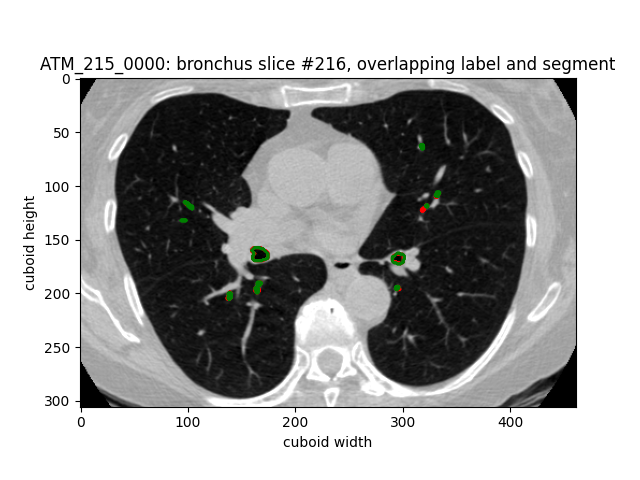
\includegraphics[width=0.3\textwidth]{results/baseline/val060/ATM_215_0000_bronchus_segmentation_slice216_at_val_epoch60} &
            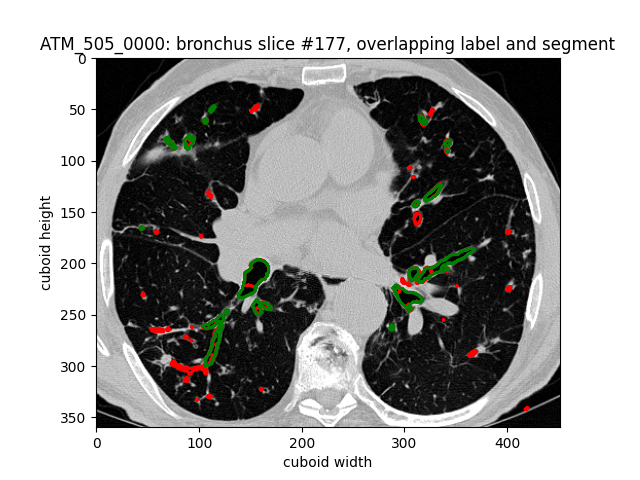
\includegraphics[width=0.3\textwidth]{results/baseline/val060/ATM_505_0000_bronchus_segmentation_slice177_at_val_epoch60} &
            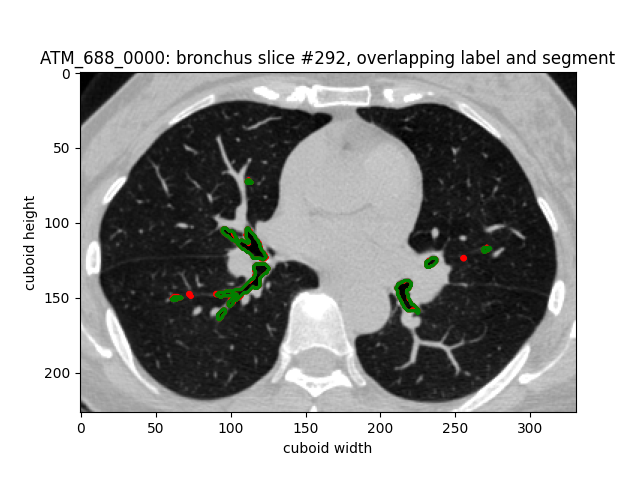
\includegraphics[width=0.3\textwidth]{results/baseline/val060/ATM_688_0000_bronchus_segmentation_slice292_at_val_epoch60} \\
            FPR = 0.021\%           & FPR = 0.026\%             & FPR = 0.05\% \\
            FNR = 18.069\%          & FNR = 44.246\%             & FNR = 2.038\% \\
            Sensitivity = 81.931\%  & Sensitivity = 55.754\%    & Sensitivity = 97.962\% \\
            Precision = 90.068\%    & Precision = 72.892\%      & Precision = 94.411\% \\
            DSC = 85.81\%           & DSC = 63.18\%             & DSC = 96.15\% \\
            \hline
        \end{tabular}
    \end{table}
    
    需要说明的是,表\ref{tbl:hcomparison_metrics}中的指标数据是基于当前切片计算的,不是基于整个气道树来计算的,因此就不
    带有BD和TLD两个指标的数据了。还有一点,切片图像中由绿色像素框起来的区域是真实的气管,红色的像素是分割出来的。绿色像素覆盖
    在红色像素上,对于没有覆盖住而露出来的红色像素是假阳性的。
    
    \item[B.] 在纵向对比时,我们挑选ATM\_054\_0000这个病例,将第10个迭代周期,第20/30/40/50/60个迭代周期里的Slice
    \#264拿出来对比,看看它们的分割效果和指标数据,如表\ref{tbl:vcomparison_metrics}所示。
    \begin{table}[ht]
        \bicaption[验证集ATM\_054\_0000病例第264张切片图像分割效果与指标纵向比较]
            {验证集ATM\_054\_0000病例第264张切片图像分割效果与指标纵向比较}
            {Vertical comparison of segmentation and metrics for ATM\_054\_0000 slice \#264}
        \label{tbl:vcomparison_metrics}
        \centering
        \begin{tabular}{|c|c|c|}
            \hline
            ATM\_054\_0000 & ATM\_054\_0000 & ATM\_054\_0000 \\
            Epoch \#10 & Epoch \#20 & Epoch \#30 \\
            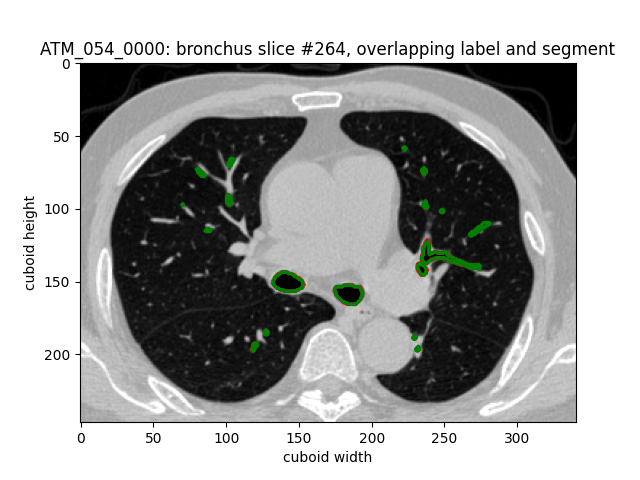
\includegraphics[width=0.3\textwidth]{results/baseline/val010/ATM_054_0000_bronchus_segmentation_slice264_at_val_epoch10} &
            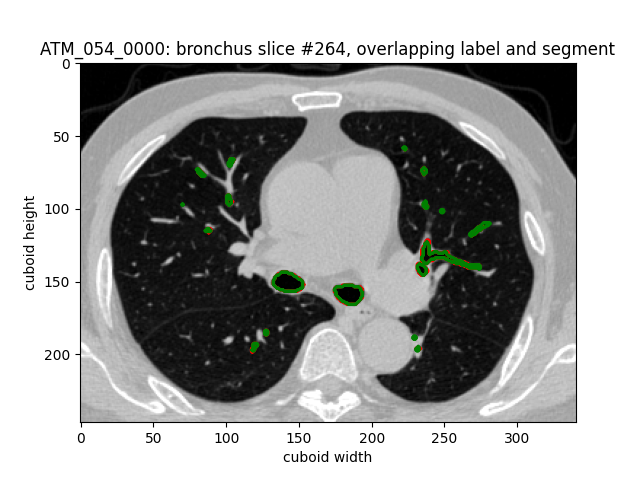
\includegraphics[width=0.3\textwidth]{results/baseline/val020/ATM_054_0000_bronchus_segmentation_slice264_at_val_epoch20} & 
            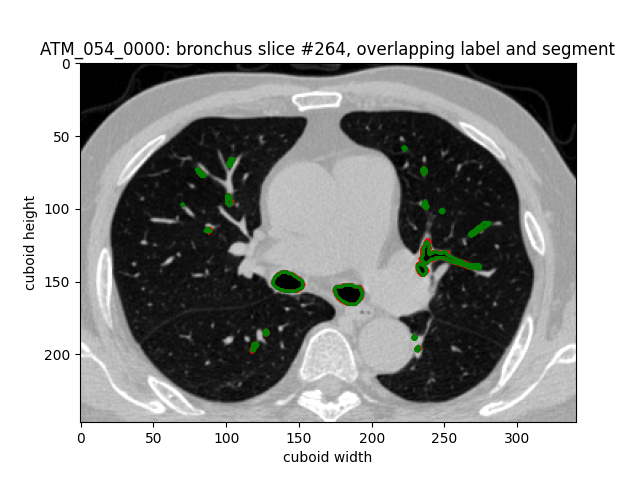
\includegraphics[width=0.3\textwidth]{results/baseline/val030/ATM_054_0000_bronchus_segmentation_slice264_at_val_epoch30} \\
            FPR = 0.025\%           & FPR = 0.061\%             & FPR = 0.066\% \\
            FNR = 12.268\%          & FNR = 6.419\%             & FNR = 6.419\% \\
            Sensitivity = 87.732\%  & Sensitivity = 93.581\%    & Sensitivity = 93.581\% \\
            Precision = 96.698\%    & Precision = 92.786\%      & Precision = 92.264\% \\
            DSC = 92.0\%            & DSC = 93.18\%             & DSC = 92.92\% \\
            \hline
            ATM\_054\_0000 & ATM\_054\_0000 & ATM\_054\_0000 \\
            Epoch \#40 & Epoch \#50 & Epoch \#60 \\
            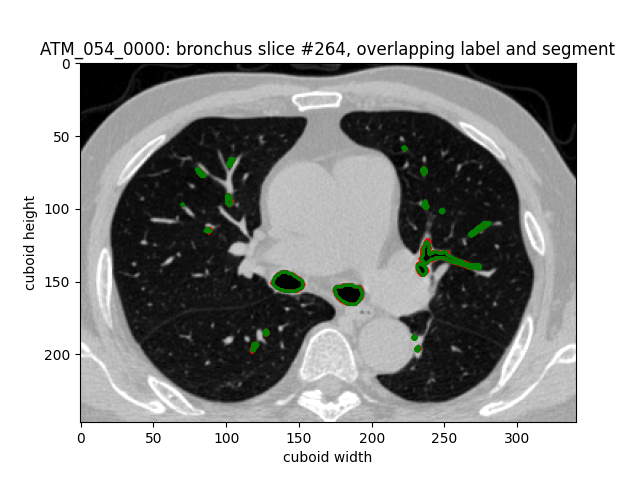
\includegraphics[width=0.3\textwidth]{results/baseline/val040/ATM_054_0000_bronchus_segmentation_slice264_at_val_epoch40} &
            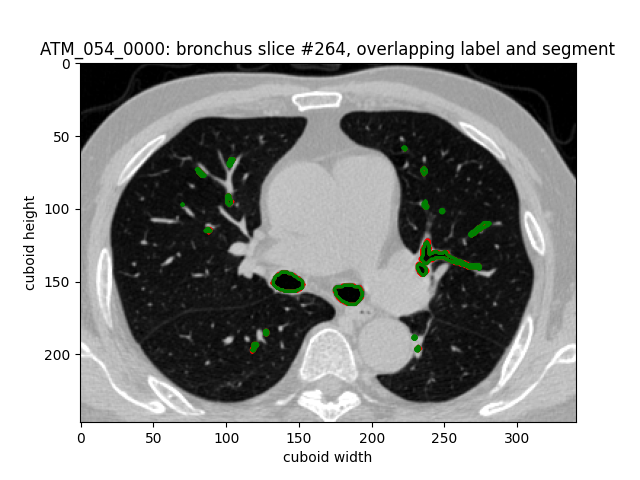
\includegraphics[width=0.3\textwidth]{results/baseline/val050/ATM_054_0000_bronchus_segmentation_slice264_at_val_epoch50} & 
            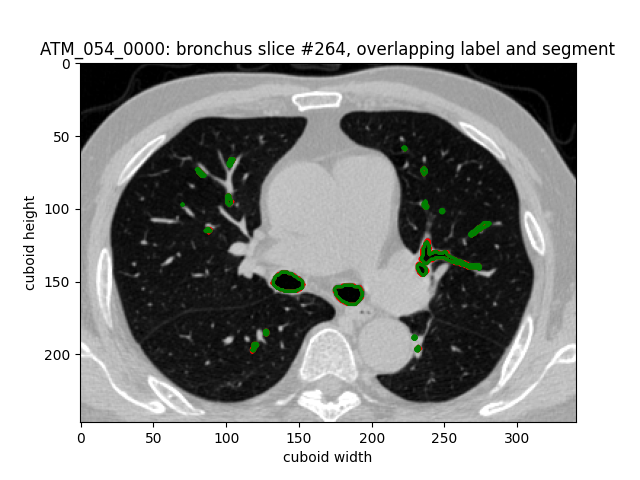
\includegraphics[width=0.3\textwidth]{results/baseline/val060/ATM_054_0000_bronchus_segmentation_slice264_at_val_epoch60} \\
            FPR = 0.066\%          & FPR = 0.068\%             & FPR = 0.068\% \\
            FNR = 6.277\%          & FNR = 6.277\%             & FNR = 5.991\% \\
            Sensitivity = 93.723\% & Sensitivity = 93.723\%    & Sensitivity = 94.009\% \\
            Precision = 92.275\%   & Precision = 92.017\%      & Precision = 92.039\% \\
            DSC = 92.99\%          & DSC = 92.86\%             & DSC = 93.01\% \\
            \hline
        \end{tabular}
    \end{table}

\end{enumerate}

从表\ref{tbl:hcomparison_metrics}看,ATM\_174\_0000 Slice \#74的Sensitivity和DSC两项指标表现得最差,这是因为
该CT图像的切片数量最少,其支气管气道明显狭窄,可能患有肺部疾病。倒数第二差的是ATM\_505\_0000 Slice \#177这张切片,存在
很多红色的像素表明假阴性像素很多,它们通常是一些比较细小的支气管。分割网络遗漏掉了这些真实存在的支气管体素。在这9例CT切片图像
中分割最好的当属于ATM\_688\_0000 Slice \#292, Sensitivity, Precision, DSC分别取得了97.62\%, 94.411\%, 96.15\%
的高分。这表明分割网络对于肺叶支气管、段支气管这种中等管腔直径的支气管能很清晰地分割出来。

从表\ref{tbl:vcomparison_metrics}看,随着训练的持续进行,从第20个迭代周期开始,分割性能就逐渐开始稳定下来。Sensitivity,
Precision和DSC都已经达到了92\%以上的优秀表现。不管是对于左右肺主气管、肺叶支气管,还是很细小的段支气管都可能清晰地分割出来,
证明3D-UNet基准网络性能基本上能达到临床应用的水平。

最后我们来看看3D-UNet网络对整个支气管气道树的分割表现。对于测试集的19例CT图像的分割,其性能指标如表
\ref{tbl:testset_airway_tree_metrics}所示。其中打下划线强调的表示在当前指标表现最出色的。
\begin{table}[ht]
    \bicaption[测试集上3D-UNet基准网络对支气管气道树分割的性能指标表现]
        {测试集上3D-UNet基准网络对支气管气道树分割的性能指标表现}
        {The metrics table of 3D-UNet baseline model segmenting airway tree in testset}
    \label{tbl:testset_airway_tree_metrics}
    \centering
    \begin{tabular}{cccccccc}
        \toprule
        病例名称          & FPR           & FNR            & Sensitivity     & Precision      & DSC           & BD            & TLD           \\
        \midrule
        ATM\_001\_0000 & \uline{0.006} & 7.24           & 92.76           & \uline{98.089} & 95.35         & 68.95         & 84.17         \\
        ATM\_024\_0000 & 0.031         & 7.236          & 92.764          & 90.916         & 91.83         & 84.18         & 92.86         \\
        ATM\_034\_0000 & 0.022         & 3.705          & 96.295          & 96.251         & 96.27         & 90.75         & 93.93         \\
        ATM\_041\_0000 & 0.047         & 4.808          & 95.192          & 87.189         & 91.02         & 82.38         & 90.38         \\
        ATM\_060\_0000 & 0.024         & 2.534          & 97.466          & 93.12          & 95.24         & 88.03         & 92.72         \\
        ATM\_061\_0000 & 0.028         & 3.121          & 96.879          & 91.897         & 94.32         & 86.15         & 90.8          \\
        ATM\_074\_0000 & 0.053         & 3.838          & 96.162          & 87.038         & 91.37         & 80.49         & 89.86         \\
        ATM\_075\_0000 & 0.023         & 4.633          & 95.367          & 93.65          & 94.5          & 81.13         & 88.56         \\
        ATM\_080\_0000 & 0.026         & 4.067          & 95.933          & 93.183         & 94.54         & 76.9          & 88.11         \\
        ATM\_150\_0000 & 0.082         & 3.902          & 96.098          & 80.036         & 87.33         & 72.12         & 87.62         \\
        ATM\_158\_0000 & 0.044         & 3.461          & 96.539          & 86.953         & 91.5          & 80.75         & 90.48         \\
        ATM\_163\_0000 & 0.035         & 4.301          & 95.699          & 91.958         & 93.79         & 83.23         & 91.34         \\
        ATM\_197\_0000 & 0.032         & 9.234          & 90.766          & 90.81          & 90.79         & 59.71         & 78.46         \\
        ATM\_245\_0000 & 0.038         & \uline{0.309}  & \uline{99.691}  & 83.496         & 90.88         & \uline{100}   & \uline{100}   \\
        ATM\_246\_0000 & 0.04          & 0.611          & 99.389          & 82.853         & 90.37         & \uline{100}   & \uline{100}   \\
        ATM\_260\_0000 & 0.016         & 1.041          & 98.959          & 94.227         & \uline{96.53} & 98.34         & 97.93         \\
        ATM\_266\_0000 & 0.019         & 2.351          & 97.649          & 93.112         & 95.33         & 99.38         & 98.39         \\
        ATM\_271\_0000 & 0.049         & 1.044          & 98.956          & 86.544         & 92.33         & 97.6          & 97.62         \\
        ATM\_638\_0000 & 0.014         & 3.152          & 96.848          & 95.199         & 96.02         & 90.48         & 95.45         \\
        \bottomrule
    \end{tabular}
\end{table}
从表\ref{tbl:testset_airway_tree_metrics}可以看出,ATM\_245\_0000这一例CT图像分割表现最好,BD和TLD两个指标竟然
达到例100\%, 这说明已经将支气管气道树中的分支全部检测出来,也获得了最长的分支中心线长度之和。

对于验证集的9例CT图像,我们不仅要展示支气管气道树分割的可视化结果,如表\ref{tbl:visualize_airway_3d_model}所示。
\begin{table}[!htp]
    \bicaption[验证集9例CT图像的支气管气道树分割可视化3D模型]
        {验证集9例CT图像的支气管气道树分割可视化3D模型}
        {Visualize the airway 3D model of 9 CT cases in validateset}
    \label{tbl:visualize_airway_3d_model}
    \centering
    \begin{tabular}{|c|c|c|}
        \hline
        ATM\_029\_0000 & ATM\_054\_0000 & ATM\_055\_0000 \\
        \hline
        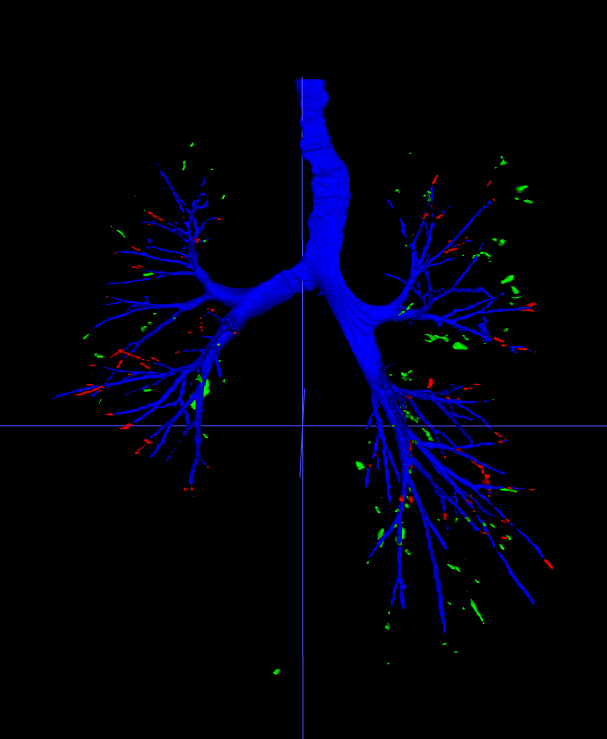
\includegraphics[width=0.3\textwidth]{results/baseline/validate/ATM_029_0000_airway_tree_with_3colors_at_val_epoch1} &
        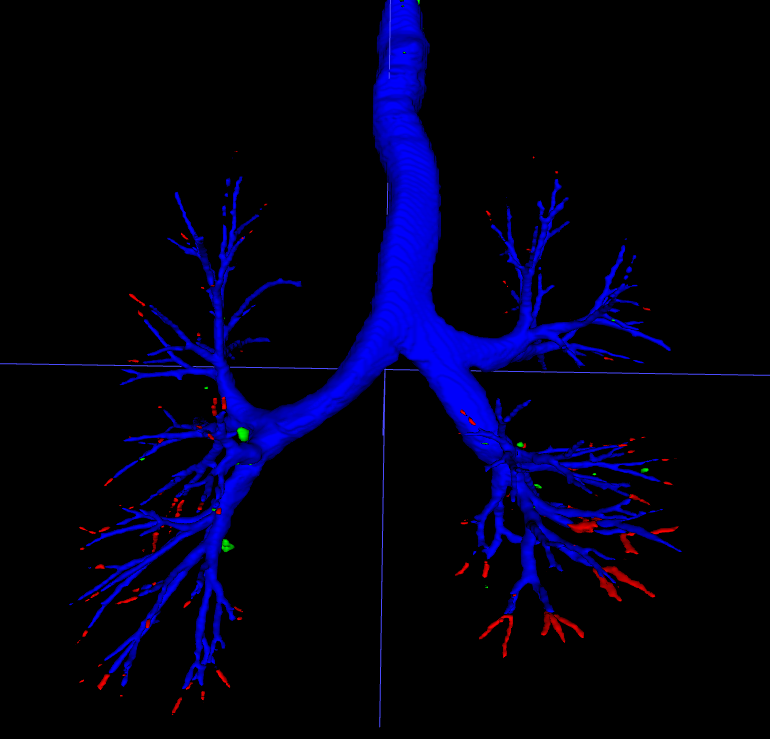
\includegraphics[width=0.3\textwidth]{results/baseline/validate/ATM_054_0000_airway_tree_with_3colors_at_val_epoch1} &
        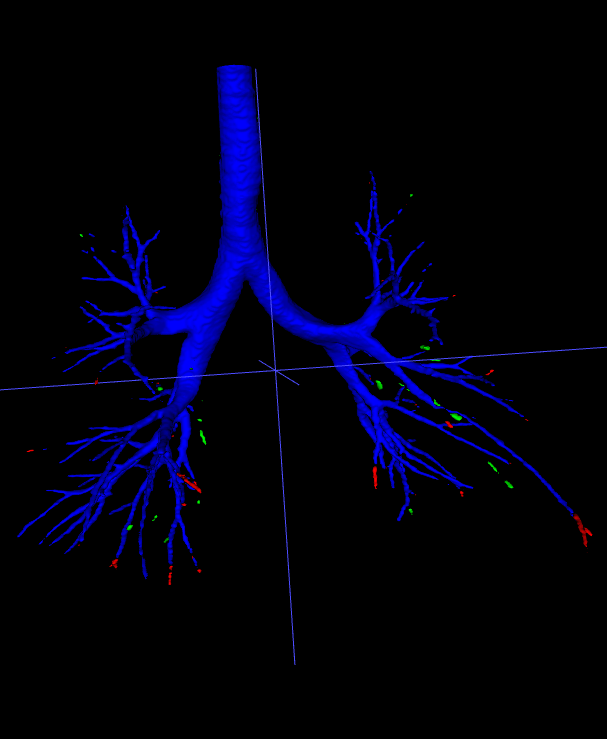
\includegraphics[width=0.3\textwidth]{results/baseline/validate/ATM_055_0000_airway_tree_with_3colors_at_val_epoch1} \\
        \hline
        ATM\_057\_0000 & ATM\_091\_0000 & ATM\_174\_0000 \\
        \hline
        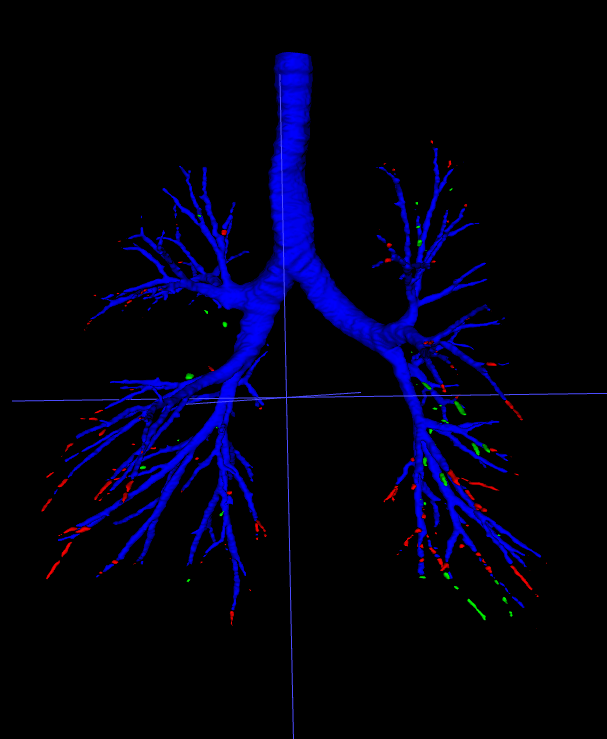
\includegraphics[width=0.3\textwidth]{results/baseline/validate/ATM_057_0000_airway_tree_with_3colors_at_val_epoch1} &
        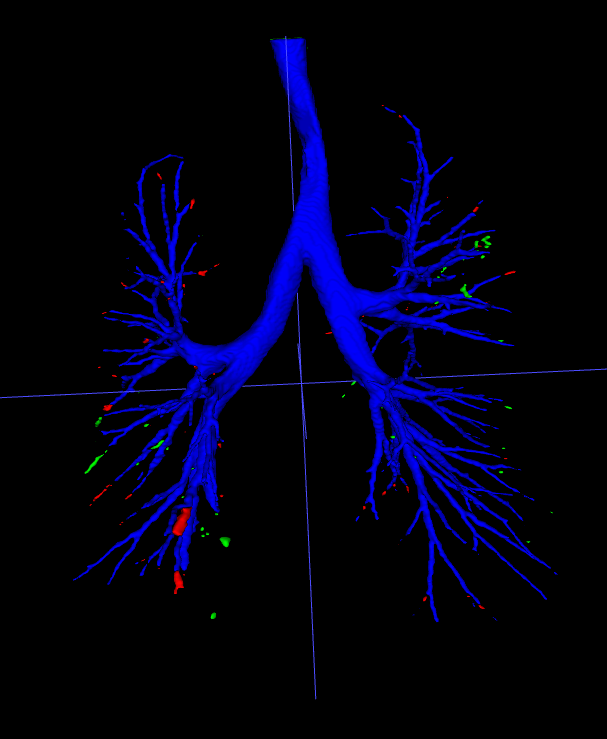
\includegraphics[width=0.3\textwidth]{results/baseline/validate/ATM_091_0000_airway_tree_with_3colors_at_val_epoch1} &
        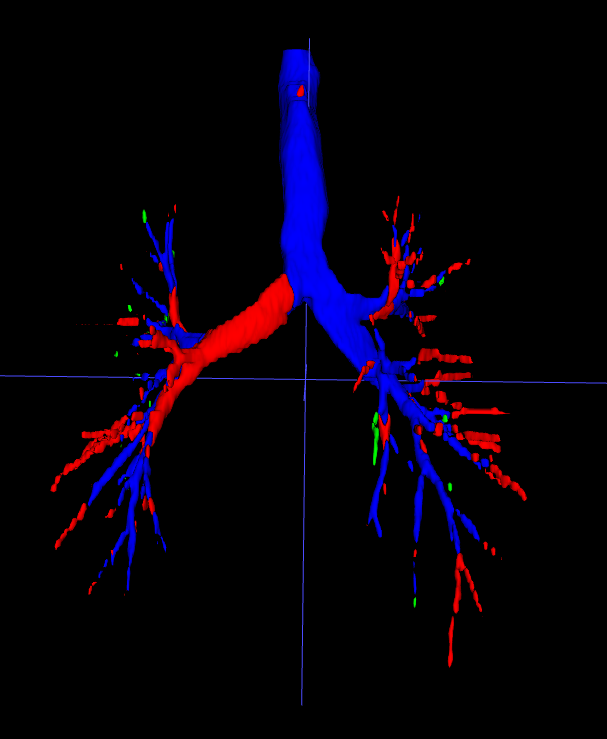
\includegraphics[width=0.3\textwidth]{results/baseline/validate/ATM_174_0000_airway_tree_with_3colors_at_val_epoch1} \\
        \hline
        ATM\_215\_0000 & ATM\_505\_0000 & ATM\_688\_0000 \\
        \hline
        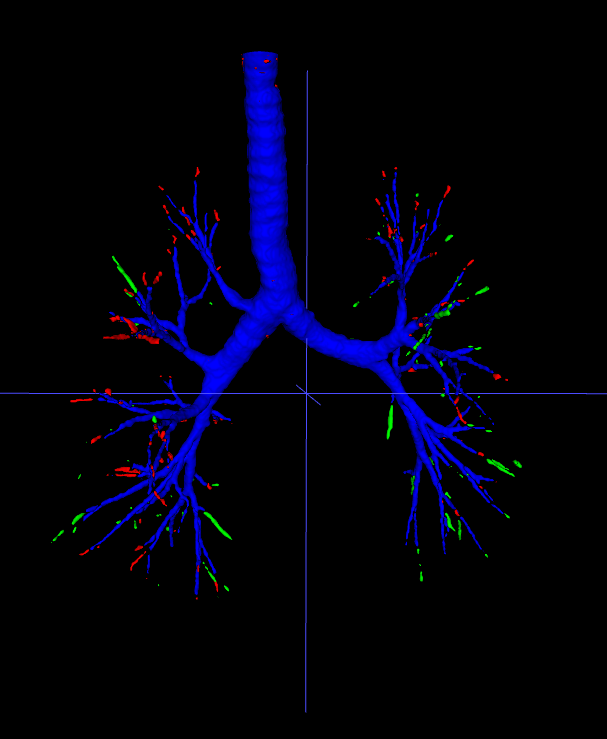
\includegraphics[width=0.3\textwidth]{results/baseline/validate/ATM_215_0000_airway_tree_with_3colors_at_val_epoch1} &
        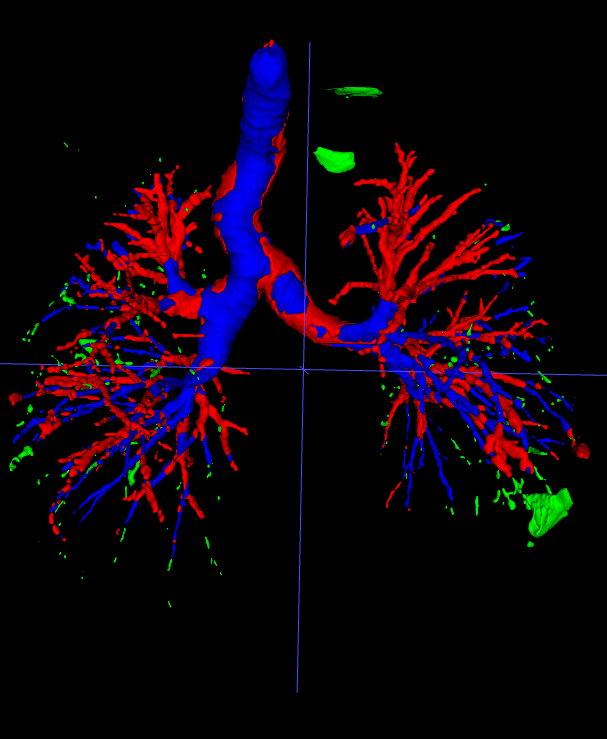
\includegraphics[width=0.3\textwidth]{results/baseline/validate/ATM_505_0000_airway_tree_with_3colors_at_val_epoch1} &
        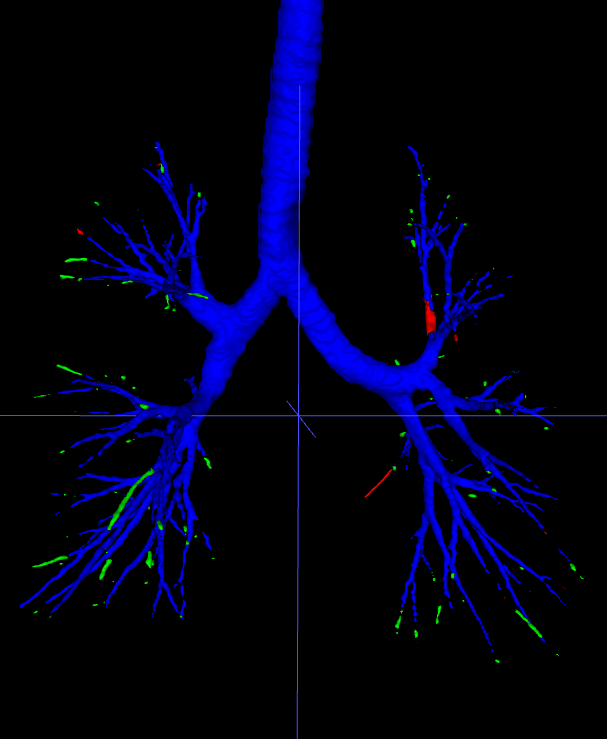
\includegraphics[width=0.3\textwidth]{results/baseline/validate/ATM_688_0000_airway_tree_with_3colors_at_val_epoch1} \\
        \hline
    \end{tabular}
\end{table}
还有完整的指标数据,见表\ref{tbl:validateset_airway_tree_metrics}。
\begin{table}[!htp]
    \bicaption[验证集9例CT图像的支气管气道树分割指标]
        {验证集9例CT图像的支气管气道树分割指标}
        {The segmentation metrics of 9 CT cases in validateset}
    \centering
    \label{tbl:validateset_airway_tree_metrics}
\begin{tabular}{cccccccc}
        \toprule
        病例名称          & FPR           & FNR            & Sensitivity     & Precision      & DSC           & BD            & TLD           \\
        \midrule
        ATM\_029\_0000 & 0.017           & 9.222          & 90.778          & 93.232         & 91.99         & 80.34         & 88.48         \\
        ATM\_054\_0000 & 0.032           & 3.876          & 96.124          & 93.343         & 94.71         & 76.78         & 85.61         \\
        ATM\_055\_0000 & 0.031           & 3.571          & 96.429          & 91.66          & 93.98         & 82.51         & 89.9          \\
        ATM\_057\_0000 & 0.03            & 5.757          & 94.243          & 92.35          & 93.29         & 72.85         & 84.36         \\
        ATM\_091\_0000 & 0.034           & 3.432          & 96.568          & 91.148         & 93.78         & 84.04         & 91.09         \\
        ATM\_174\_0000 & 0.019           & 26.864         & 73.136          & 94.026         & 82.28         & \colorbox{red}{32.38}         & \colorbox{red}{47.19}         \\
        ATM\_215\_0000 & 0.023           & 9.419          & 90.581          & 91.951         & 91.26         & 73.3          & 84.83         \\
        ATM\_505\_0000 & 0.05            & 55.899         & 44.101          & 84.808         & 58.03         & \colorbox{red}{21.5}          & \colorbox{red}{39.1}          \\
        ATM\_688\_0000 & 0.023           & 2.217          & 97.783          & 93.409         & 95.55         & 93.07         & 95.73         \\
        \bottomrule
    \end{tabular}
\end{table}
在表\ref{tbl:visualize_airway_3d_model}中我们看到ATM\_174\_0000和ATM\_505\_0000两个病例中出现大量的红色的假阴性
体素。结合表\ref{tbl:validateset_airway_tree_metrics}中这两个病例的BD、TLD两项指标低至30\%的不正常现象\footnote{
表\ref{tbl:validateset_airway_tree_metrics}中红色标记的数据},而Precision
能够达到90\%以上。纵览这9张气道树3D分割图,其他7张图都没有在气管、左右肺主气管发生漏检。 
所以,我们推断ATM\_174\_0000和ATM\_505\_0000两个病例的支气管气道树异常的原因可能是:
\begin{enumerate}
    \item[a)] 图像异位,做标注工作的临床医生没有看到明确的支气管管壁边缘而没有标注;
    \item[b)] 患者有严重的肺部疾病,支气管管壁破裂或缺失。
\end{enumerate}
我们更倾向于后者。

在此需要强调一点,我们是将3D-UNet作为我们的基准网络,所以在此没有做消融研究Ablation Study,没有凸显3D-UNet网络比其他
已知网络更优秀。从上述的实验结果展示和分析,我们认识到3D-UNet网络存在不足之处,后面的章节以3D-UNet网络为基础,在此之上进行
改进。

\section{本章小结}

本章详细讲述了3D-UNet这一基准网络,我们在基于CT扫描图像的支气管气道树分割任务中采用3D-UNet网络来对肺部支气管进行分割,我们
使用Python语言与PyTorch深度学习框架设计实现了一个3D-UNet分割网络,针对ATM22数据集进行特定的优化设计。我们在上海交通大学
高性能计算中心的AI超算上训练网络,训练完成后在验证集和测试集上输出完整的支气管气道树三维模型和评价指标数据。我们展示了实验结果,
可视化显示支气管气道树的3D模型,分析这些实验数据,并对两个明显异常的病例进行分析推断异常的产生原因。

通过以上实验证明了3D-UNet网络可以胜任三维支气管气道树的分割任务,但在精度准确率、FPR和DSC等指标方面还不够,需要进一步改进3D-UNet
网络。后文在此实验的基础上研究如何改进该网络,以更好更精确地分割支气管气道树三维模型。
